\documentclass[12pt,twoside]{article}
	\clearpage{}\usepackage{lmodern}
\usepackage[T1]{fontenc}
\usepackage[polish]{babel}
\usepackage[utf8]{inputenc}
\usepackage{hyperref}
\hypersetup{pdftex,colorlinks=true,allcolors=black}
\usepackage{hypcap}
\usepackage{indentfirst}
\usepackage[style=numeric-comp,sorting=none,firstinits=true]{biblatex}
\usepackage{csquotes}
\DeclareQuoteStyle[quotes]{polish}
  {\quotedblbase}
  {\textquotedblright}
  [0.05em]
  {\quotesinglbase}
  {\fixligatures\textquoteright}
\DeclareQuoteAlias[quotes]{polish}{polish}
\DeclareQuoteOption{polish}

\usepackage{graphicx}
\selectlanguage{polish}
\providecommand{\tightlist}{  \setlength{\itemsep}{0pt}\setlength{\parskip}{0pt}}
\usepackage[a4paper,inner=3.5cm,outer=2.5cm]{geometry}
\usepackage{import}
\graphicspath{{graphics/}}
\usepackage{listings}
\usepackage{color}
\definecolor{lightgray}{rgb}{.9,.9,.9}
\definecolor{darkgray}{rgb}{.4,.4,.4}
\definecolor{purple}{rgb}{0.65, 0.12, 0.82}

\lstdefinelanguage{JavaScript}{
  keywords={typeof, new, true, false, catch, function, return, null, catch, switch, var, if, in, while, do, else, case, break},
  keywordstyle=\color{blue}\bfseries,
  ndkeywords={class, export, boolean, throw, implements, import, this},
  ndkeywordstyle=\color{darkgray}\bfseries,
  identifierstyle=\color{black},
  sensitive=false,
  comment=[l]{//},
  morecomment=[s]{/*}{*/},
  commentstyle=\color{purple}\ttfamily,
  stringstyle=\color{red}\ttfamily,
  morestring=[b]',
  morestring=[b]"
}

\lstset{
   language=JavaScript,
   backgroundcolor=\color{lightgray},
   extendedchars=true,
   basicstyle=\footnotesize\ttfamily,
   showstringspaces=false,
   showspaces=false,
   numbers=left,
   numberstyle=\footnotesize,
   numbersep=9pt,
   tabsize=2,
   breaklines=true,
   showtabs=false,
   captionpos=b
}

\lstdefinelanguage{Elixir}{
  keywords={typeof, new, true, false, catch, function, return, null, catch, switch, var, if, in, while, do, else, case, break, rescue, after},
  keywordstyle=\color{blue}\bfseries,
  ndkeywords={defmodule, def, defp, defmacro, import, do, end, class, export, boolean, throw, implements, import, this},
  ndkeywordstyle=\color{darkgray}\bfseries,
  identifierstyle=\color{black},
  sensitive=false,
  comment=[l]{//},
  morecomment=[s]{/*}{*/},
  commentstyle=\color{purple}\ttfamily,
  stringstyle=\color{red}\ttfamily,
  morestring=[b]',
  morestring=[b]"
}

\lstset{
   language=Elixir,
   backgroundcolor=\color{lightgray},
   extendedchars=true,
   basicstyle=\footnotesize\ttfamily,
   showstringspaces=false,
   showspaces=false,
   numbers=left,
   numberstyle=\footnotesize,
   numbersep=9pt,
   tabsize=2,
   breaklines=true,
   showtabs=false,
   captionpos=b
}
\usepackage{longtable}
\usepackage{booktabs}\clearpage{}
	\bibliography{biblio} 
\begin{document}
	\clearpage{}\begin{titlepage}
	\centering
	{\scshape\LARGE Politechnika Krakowska 
	\break im. Tadeusza Kościuszki \par}
	\vspace{0.5cm}
	{\large Wydział Inżynierii Elektrycznej i Komputerowej\par}
	\vspace{1cm}
	{\scshape\LARGE Praca inżynierska\par}
	\vspace{1.5cm}
	{\LARGE\bfseries Porównanie klasycznych stosów programistycznych z nowoczesnym podejściem do budowy oprogramowania.\par}
	\vspace{1.5cm}
	{\LARGE\itshape Patryk Żmigrodzki\par}
	\vspace{1cm}

	\vfill
	
								\large
				\emph{Promotor}\\
				prof. dr hab. inż. Volodymyr Samotyy
																							
	\vfill

	{\large Kraków, 2016\par}
\end{titlepage}\clearpage{}
	\tableofcontents
	
	\clearpage{}\section{Wstęp}\label{wstux119p}

Rozwój jest koniecznym i nieodłącznym elementem każdej branży. W tak
dynamicznie rozwijającej się dziedzinie jaką jest informatyka
szczególnie ważne jest aby nie dopuścić do stagnacji, zachować
konkurencyjność. Innowacyjność na polu programistycznym może okazać się
kartą przetargową do uzyskania przewagi w określonym sektorze. Z drugiej
strony optymistyczne i pochopne podejście do nowości, zbyt wczesna
adaptacja niedojrzałych lub niestabilnych technologii może doprowadzić
do poważnych komplikacji.\\
Przedmiotem tej pracy jest zbadanie nowych technologii w zastosowaniach
biznesowych. W celu porównania przydatności i potencjału
technologicznego wydzielono dwie grupy. Do pierwszej z nich należą
środowiska cieszące się dobrą reputacją, z ustaloną pozycją na rynku,
zaś do drugiej rozwiązania nowe, promujące odmienne modele modele
programowania. Dokonano porównania na płaszczyźnie współczesnych
problemów systemów informatycznych. Poruszono tematy architektury takich
systemów jako istotnego czynnika w tworzeniu udanych projektów
programistycznych. Równie znaczącym zagadnieniem jest efektywne
wykorzystanie dostępnego sprzętu komputerowego poprzez przetwarzanie
wieloprocesorowe. Z tego względu przyjrzano się różnym podejściom i
modelom współbieżności, wykorzystywanym przez testowane technologie.
Jednakże, możliwości równoczesnego przetwarzania nie kończą się na
pojedynczej maszynie. Zastosowanie architektur rozproszonych jest równie
ważną cechą współczesnych systemów informatycznych. Poza zbadaniem
aspektów skalowalności przetestowano wydajność wybranych technologii w
typowych dla współczesnych systemów informatycznych scenariuszach
użytkowania. Poddano je również analizie pod względem efektywności pracy
programistycznej, będącej kluczowym czynnikiem w procesie tworzenia
oprogramowania.
\clearpage{}
	\clearpage{}\section{Opis technologii}\label{opis-technologii}

Współczesne języki programowania to nie tylko składania i kompilatory.
To także ustalone modele i wzorce programistyczne, standardy oraz
społeczności.\\
Typowym przedstawicielem kategorii klasycznych technologii jest Java, ze
względu na powszechność, długą historię oraz wyraźne podłoże biznesowe.
Do drugiej, innowacyjnej, grupy wybrano dwa języki programowania:
skupiający ogromną społeczność programistów JavaScript wraz z Node.js
oraz promujący funkcyjną metodykę programowania Elixir.

\subsection{Java}\label{technologie---java}

Java jest platformą programistyczną, której kluczowymi elementami są:
obiektowy język programowania Java oraz Java Virtual Machine (ang.
wirtualna maszyna Javy). Została stworzona w 1995 przez firmę Sun
Microsystems do budowania przenośnego oprogramowania. Obecnie jest ona
własnością Oracle Corporation. Java należy do jednych z
najpopularniejszych języków programowania na
świecie\autocite{tiobe2015index}. Dzieli się ona na kilka wydań
różniących się funkcjonalnością i przeznaczeniem. Najbardziej powszechne
z nich to \emph{Java Standard Edition} przeznaczone do zastosowań
ogólnych. Stanowi ona rdzeń języka wzbogacony o często wykorzystywane
biblioteki jak dostęp do bazy danych czy łączność sieciową oraz
narzędzia, w skład których wchodzą wirtualna maszyna i aplikacje
deweloperskie.\\
Kolejnym wydaniem jest \emph{Java Micro Edition} cechująca się małymi
wymaganiami sprzętowymi, przeznaczona do programowania systemów
wbudowanych. Rozbudowaną bibliotekę edycji standardowej zastąpiono
mechanizmami niezbędnymi do interakcji z warstwą sprzętową. Ostatnim z
nich jest \emph{Java Enterprise Edition}. Bazuje ono na Javie SE,
rozszerzając ją o interfejsy przeznaczone dla rozbudowanych,
skalowalnych systemów sieciowych do zastosowań
biznesowych.\autocite{jendrock2014jee}

\subsection{JavaScript}\label{javascript}

JavaScript jest językiem programowania zapoczątkowanym w 1995 przez
Netscape Communications Corporation do wykonywania skryptów na stronach
internetowych. Język ten bardzo się rozwinął i wyrósł ponad pierwotne
skryptowe zastosowania. Bywa nazywany językiem Internetu, gdyż jest
implementowany przez większość przeglądarek internetowych stanowiąc
warstwę logiczną stron www, obok HTML tworzącego treść i CSS
specyfikującego warstwę prezentacji.\autocite{flanagan2006javascript}

\subsubsection{Node.js}\label{node.js}

Nie wszystkie implementacje JavaScriptu są częścią przeglądarek
internetowych. Można go również zastosować do tworzenia oprogramowania
serwerowego przy użyciu środowiska Node.js. Dzięki temu programiści
rozwijający aplikacje klienckie w JavaScripcie mogą wykorzystać swoje
umiejętności do programowania logiki serwerowej. Node.js bazuje na
silniku JavaScriptowym przeglądarki Google Chrome nazywanym V8. Do
implementacji silnika oraz Node.js wykorzystano języki C oraz C++. Wybór
ten podyktowany był możliwością ograniczenia zapotrzebowania na pamięć
operacyjną przy zachowaniu wysokiej wydajności. W przeciwieństwie do
większości współczesnych środowisk programistycznych, Node do obsługi
współbieżnego przetwarzania logiki biznesowej, zamiast wielowątkowości,
wykorzystuje model oparty o asynchronicznie przetwarzane zdarzeń. Takie
połączenie miało na celu stworzenie platformy, która umożliwiałaby w
prosty sposób budowanie lekkich i wydajnych systemów informatycznych.
Dzięki powszechności JavaSciptu w przeglądarkach internetowych oraz
powstania możliwości zastosowania go po stronie serwerowej, wokół języka
zgromadziła się ogromna społeczność. Repozytorium \emph{npm} przechowuje
ponad 230 tysięcy publicznie dostępnych bibliotek oraz odnotowuje prawie
140 milionów pobranych plików
dziennie.\autocite{npm2015,tilkov2010node,lerner2011node}

\subsection{Elixir i Erlang}\label{elixir-i-erlang}

Elixir to język programowania stworzony na podstawie języka
\emph{Erlang}. Korzenie te są na tyle wyraźne i znaczące, że nie sposób
go przedstawić bez wcześniejszego zapoznania się z Erlangiem.

\subsubsection{Erlang}\label{erlang}

Erlang jest funkcyjnym językiem programowania stworzonym w latach
osiemdziesiątych przez szwedzką firmę telekomunikacyjną Ericsson.
Przeznaczeniem tej technologii było budowanie skalowalnych i
niezawodnych systemów.\\
Pomimo swoich początków w systemach telekomunikacyjnych nie jest
wyspecjalizowany w tej domenie, a sprawdza się wszędzie tam gdzie
zachodzi potrzeba współbieżności, rozproszonej komunikacji i odporności
na błędy.\autocite{armstrong96erlang} W dobie internetu są to cechy
bardzo pożądane. Aby spełnić postawione założenia stworzono wirtualną
maszynę zwaną BEAM (Bogdan/Björn's Erlang Abstract
Machine)\autocite{hebert2013erlang}. Programy pisane w Erlangu są wysoce
współbieżne ze względu na fakt, że poszczególne funkcjonalności są
wykonywane w ramach lekkich procesów (aktorów){[}zob
\ref{model-aktorowy}{]}. Ich cyklem życia zarządza wirtualna maszyna,
rozdzielając dostępne zasoby sprzętowe. Aby zapewnić niezawodność
procesy są od siebie odseparowane i niezależne, awaria jednego z nich
nie prowadzi do eskalacji problemu. Zbiór takich jednostek może tworzyć
złożone, skalowalne systemy.\autocite{logan2010erlang}

\subsubsection{Elixir}\label{elixir}

\emph{Elixir} jest młodym językiem programowania działającym na maszynie
wirtualnej \emph{Erlanga}. W przeciwieństwie do \emph{Erlanga}, nie jest
to produkt konkretnej firmy, a otwarty projekt, rozwijany przez
społeczność entuzjastów.\\
Celem José Valima, twórcy Elixira, było stworzenie rozszerzalnego oraz
przyjaznego programistom języka programowania
\autocite{valim2013design}. Pomimo tego, że Elixir jest bardzo zbliżony
do Erlanga, jest przystępniejszy dla użytkownika. Uporządkowano
standardową bibliotekę pozbywając się zbędnych, zduplikowanych elementów
oraz wprowadzono powszechne konwencje ułatwiające tworzenie i utrzymanie
kodu. Ponadto \emph{Elixir} wprowadza mechanizmy pozwalające rozszerzać
język przy użyciu metaprogramowania i polimorfizmu.\\
Dzięki wykorzystaniu BEAM, Elixir może korzystać z narzędzi oraz
bibliotek stworzonych na potrzeby Erlanga kodu bez uszczerbku na
wydajności\autocite{thomas2014elixir, stlaurent2014elixir}.
\clearpage{}
	\clearpage{}\section{Architektura systemu
informatycznego}\label{architektura-systemu-informatycznego}

Złożoność systemów informatycznych stale rośnie. Wraz ze złożonością
zwiększa się ich zapotrzebowanie na moc obliczeniową. Biorąc pod uwagę
spowalniające prawo Moore'a, sprostanie potrzebom zwiększenia mocy jest
znacznie utrudnione. Rozwiązaniem tego problemu jest stosowanie
architektur równoległych, procesorów wielordzeniowych i układów
wieloprocesorowych. Wzrost zainteresowania komputerami wielordzeniowymi
niesie dodatkową pracę programistyczną, wymagającą tworzenia
oprogramowania współbieżnego. Taki kod jest znacznie trudniejszy do
analizy, ponieważ poza kontekstem aktualnie wykonywanej sekwencji kodu
należy wziąć pod uwagę synchronizację z innymi wątkami. Poziom
komplikacji zbioru częściowo uporządkowanych operacji wykonywanych
współbieżnie jest znaczenie wyższy niż programu sekwencyjnego. Dodatkową
przeszkodą jest problem pamięci współdzielonej. Dominującym modelem
programowania współbieżnego jest wykorzystanie pamięci dzielonej
pomiędzy wiele, działających paralelnie wątków. Jeżeli co najmniej dwa z
nich jednocześnie próbują uzyskać dostęp jednego obszaru pamięci pojawia
się zjawisko \emph{wyścigu}, które może prowadzić do niespójności i
uszkodzenia danych. Istnieją metody zapobiegania takim sytuacjom,
najprostsza z nich to stosowanie blokad przy dostępie do współdzielonego
obszaru pamięci. Pomimo prostoty koncepcji, stosowanie blokad w
skomplikowanych systemach może prowadzić do dużej liczby błędów,
ponieważ nie jest to podejście naturalne dla deweloperów. Blokady
wprowadzają nowe klasy problemów jak \emph{deadlocki} i
\emph{livelocki}. Prowadzi to do powstawania oprogramowania nieodpornego
na błędy, które trudno skalować. Nieustannie wytwarzane są narzędzia
oraz nowe modele współbieżności, które mają ułatwić pracę programistom,
pomagające rozwiązać wymienione problemy z blokadami
\autocite{stutter2005software, lee2006problem}.\\
Problem rosnącego zapotrzebowania na moc obliczeniową można rozwiązać
również poprzez zastosowanie systemów rozproszonych. Za tym podejściem
przemawia wiele czynników, między innymi: geograficzne rozdystrybuowanie
źródeł i ujść informacji, krótki czasu rekcji, niższa cena komputerów,
zwiększona niezawodność. Z drugiej strony tworzenie systemów
rozproszonych niesie ze sobą te same ograniczenia i problemy dostępu do
współdzielonych zasobów jak wykorzystanie pamięci współdzielonej.
Dodatkową komplikacją w tym przypadku jest tworzenie algorytmów
korzystających z wielu maszyn jednocześnie. Klasycznym podejściem jest
wykorzystanie czasu jako podstawy opracowywania algorytmów
synchronizacji. Wprowadzenie dodatkowego czynnika jakim jest czas wynika
z opóźnień powstałych w na etapie komunikacji pomiędzy procesami
działającymi na odrębnych maszynach, jednakże dodatkowa zmienna znacznie
zwiększa złożoność i nakład pracy \autocite{lamport1978time}.

\subsection{Współczesne trendy}\label{wspuxf3ux142czesne-trendy}

\subsubsection{Architektura
mikroserwisowa}\label{architektura-mikroserwisowa}

Wiele uwagi poświęca się w ostatnim czasie tematyce zastosowania
architektury mikroserwisowej w projektach systemów informatycznych.\\
Mikroserwisowy styl architektoniczny reprezentuje podejście do
wytwarzania oprogramowania jako zboru małych usług, każda działająca
jako osobny proces, porozumiewające się za pomocą lekkich protokołów.
Usługi te są zbudowane wokół funkcjonalności biznesowych i każda z nich
jest niezależnie wdrażana przez zautomatyzowane systemy wdrożeniowe.
Założeniem jest, aby usługi w jak najmniejszym stopniu wykorzystywały
narzędzia scentralizowanego zarządzania. Implementacja każdej z usług,
jak również stosowane narzędzia są na tyle niezależne od siebie, że mogą
wykorzystywać różne języki programowania i technologie przy założeniu
jednolitego interfejsu.

\begin{figure}[!ht]
\centering
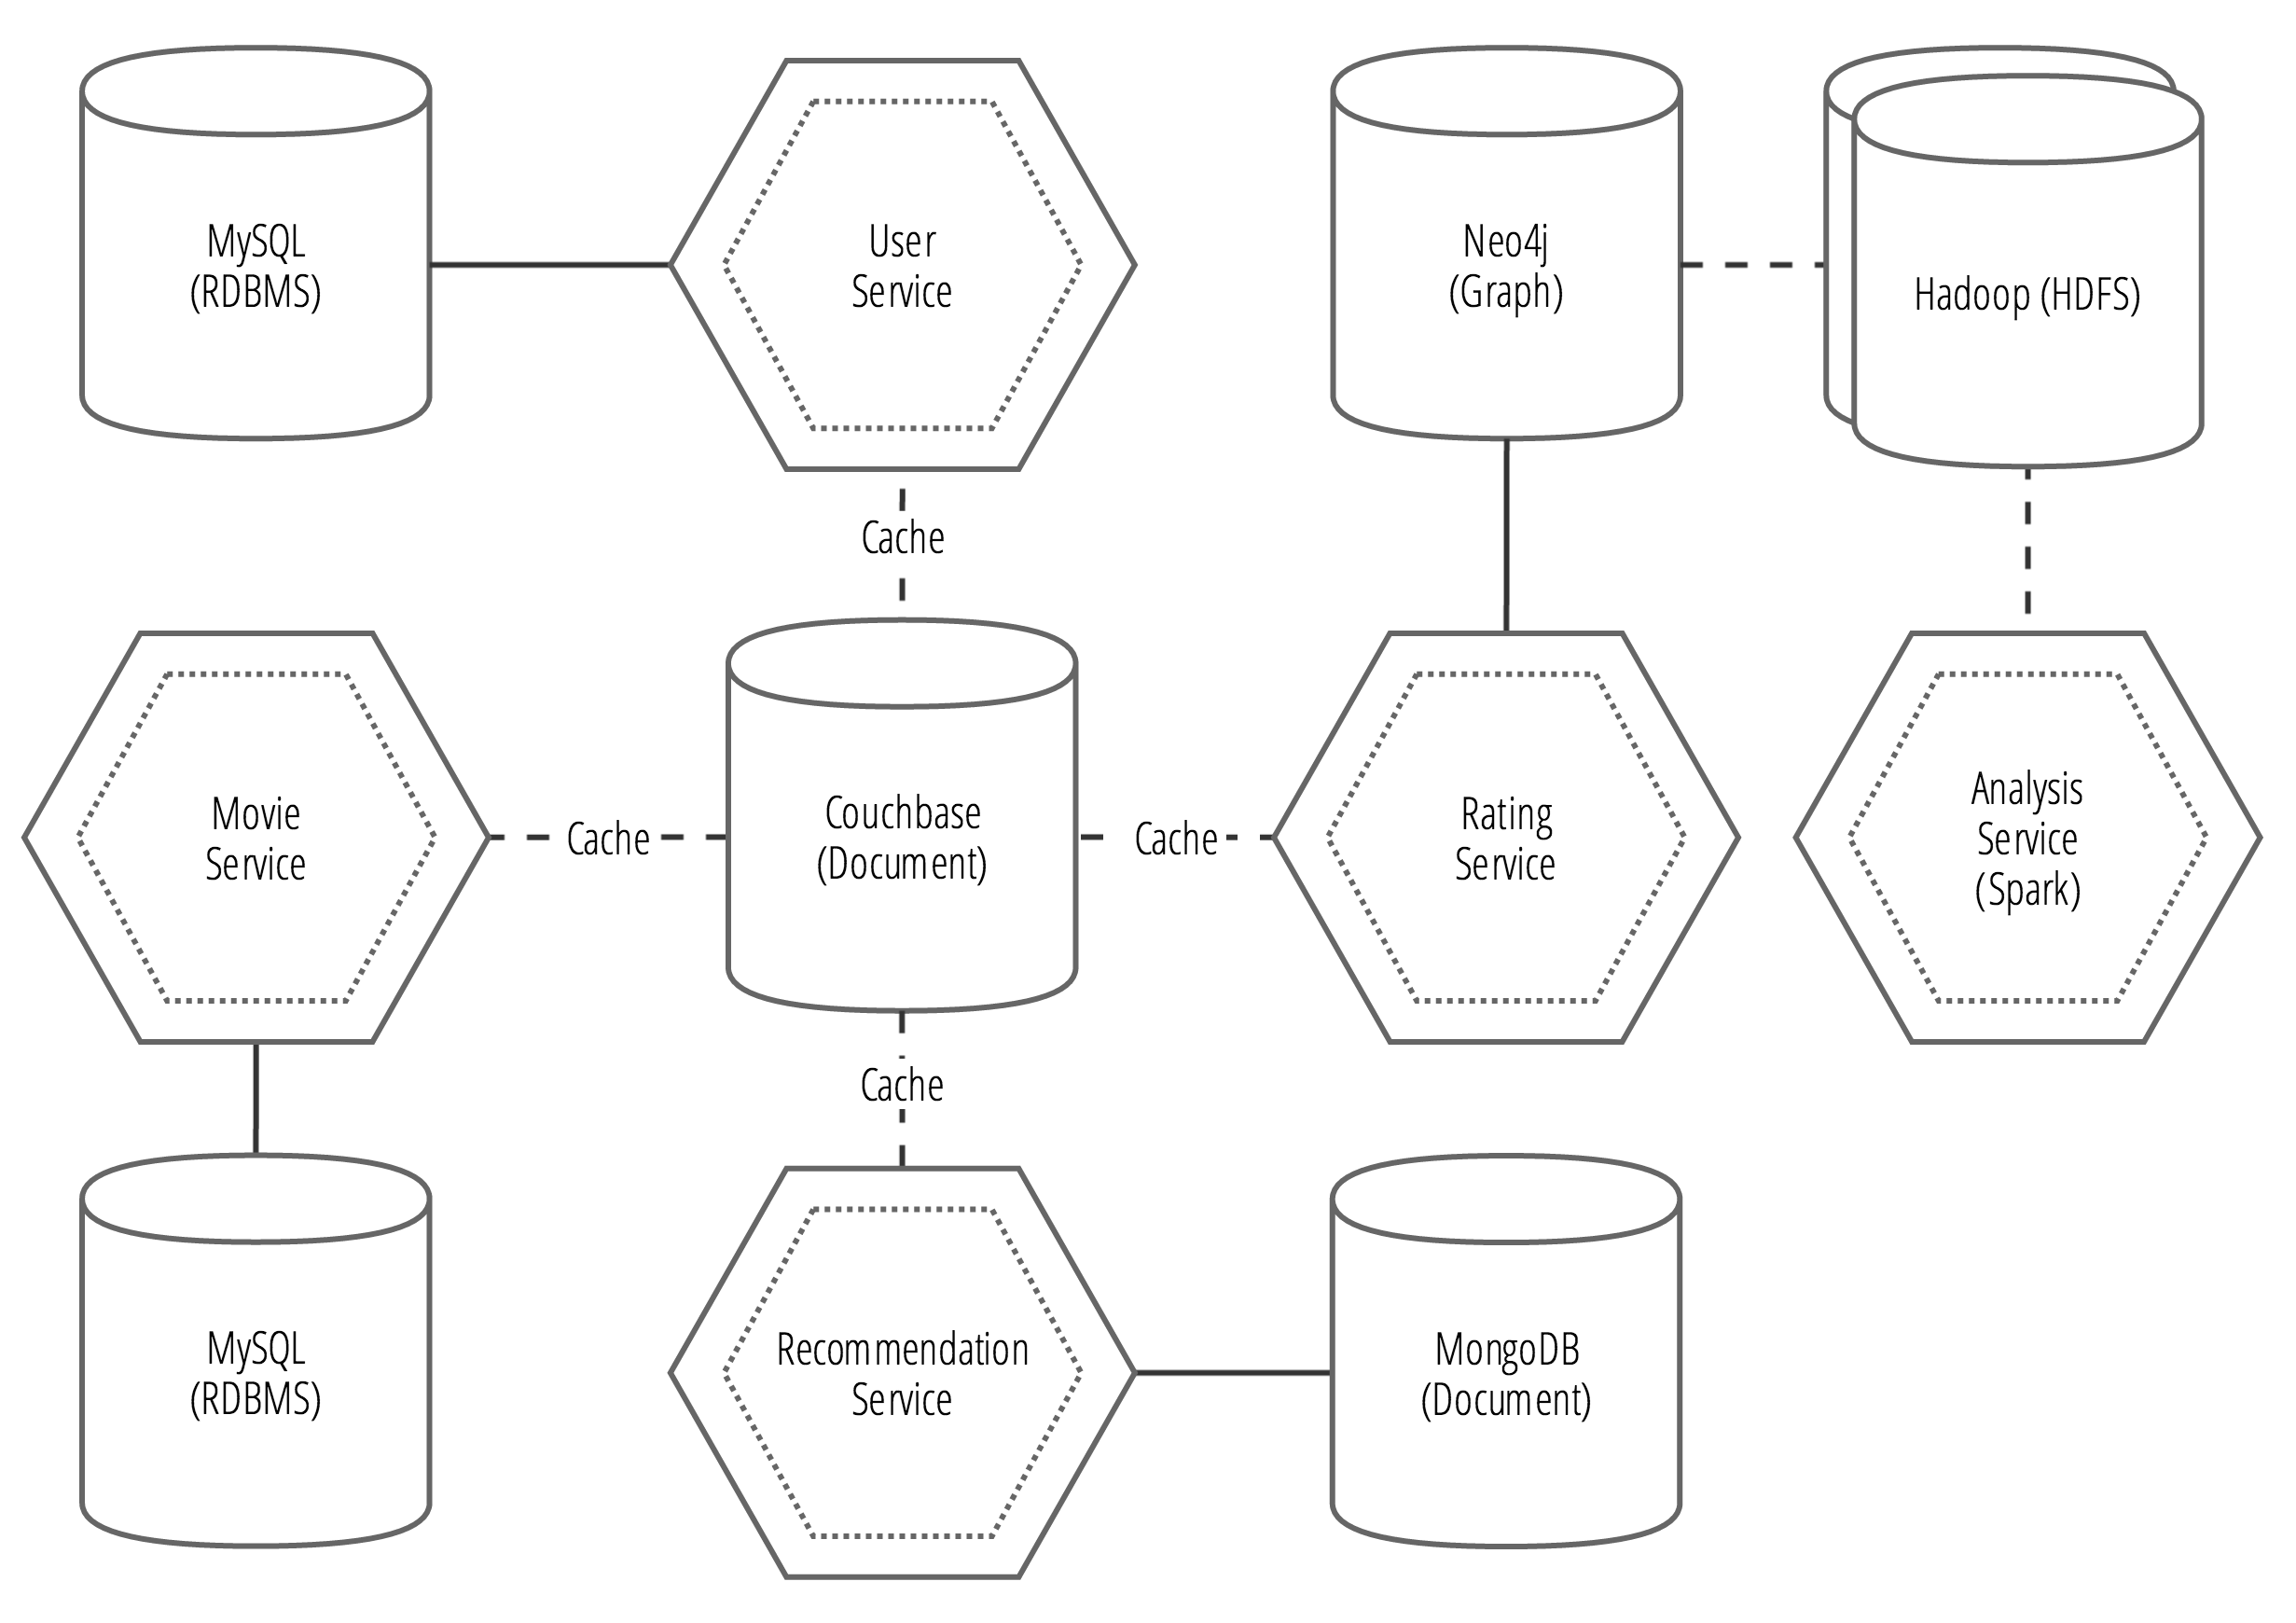
\includegraphics[resolution=500]{graphics/microservice-example.png}
\caption{Przykład projektu systemu w architekturze mikroserwisowej\autocite{bastani2015springcloud}}
\end{figure}

Nie ma formalnej definicji architektury mikroserwisowej, lecz są pewne
cechy charakterystyczne, które często pojawiają się w tego typu
systemach. Usługi często są wykorzystywane jako reużywalne komponenty.
Każdy z nich może być uruchomiony niezależnie i wprowadzanie w nich
zmian nie prowadzi do ponownego wdrożenia całości aplikacji, a jedynie
jednej z jej części. Nie tylko technologia programowania jest niezależna
od architektury, to samo tyczy się trwałych składowisk danych. Usługi
nie powinny dzielić jednej bazy danych, tak aby każda z nich była
niezależna. Nic nie stoi na przeszkodzie, aby wykorzystać różne
technologie przechowywania danych, przykładowo bazę danych relacyjną
oraz NoSQL w jednym systemie informatycznym.\\
Taki podział systemu wymaga mechanizmów zewnętrznej komunikacji pomiędzy
usługami, których koszt jest dużo wyższy od wywołań wewnątrz aplikacji.
W związku z tym funkcjonalności i odpowiedzialności muszą być
odpowiednio zaprojektowane i wydzielone. Celem tego jest minimalizacja
koniecznej komunikacji pomiędzy komponentami, co jednakże wiąże się z
dodatkowymi nakładami na projektowanie.\\
Do komunikacji w systemach rozproszonych wykorzystuje się różne
technologie i podejścia, których odpowiedni dobór ma istotne znaczenie
dla działania całości. Na przestrzeni lat stosowano wiele podejść,
przykładowo Korporacyjną Szynę Usług (ang. \emph{Enterprise Service
Bus}), która skupia szereg skomplikowanych mechanizmów zarządzania
usługami, trasowania wiadomości i transformacji danych. Społeczność
wspierająca mikroserwisy proponuje wykorzystywanie prostych, lekkich
rozwiązań komunikacyjnych. W tym celu często jest stosowany protokół
HTTP przy zastosowaniu interfejsów REST.
\autocite{fowler2014microservice, fowler2015microservices, newman2015building}

\subsection{Java}\label{architektura---java}

Architektura złożonych systemów pisanych w Javie jest silnie związana z
\emph{Javą Enterprise Edition}, gdyż definiuje ona szereg standardów dla
tworzenia logiki aplikacyjnej. Proces, w którym ustalane są owe
standardy, jest przeprowadzany w ramach \emph{Java Community Process}.
Członkami komitetu, jak również osobami biorącymi udział przy tworzeniu
propozycji, jest społeczność użytkowników Javy i specjaliści w tej
dziedzinie. Wielu z nich to przedstawiciele przedsiębiorstw aktywnie
wykorzystujących te technologie, np. Credit Suisse, Ericsson, Fujitsu,
IBM czy Intel\autocite{jcp2015}. Poprzez wkład ich oraz wielu innych
firm, Java Enterprise Edition jest powszechnie wykorzystywana między
innymi w branży finansowej czy IT do tworzenia oprogramowania
biznesowego.

\subsubsection{Architektura
wielowarstwowa}\label{architektura-wielowarstwowa}

Java EE definiuje architekturę tworzonych usług jako wielowarstwową
aplikację, mającą zapewnić skalowalność, dostępność oraz łatwość
zarządzania niezbędną dla systemów biznesowych. Przyjmując takie
założenia autorzy Javy EE podzielili logikę aplikacji na komponenty w
zależności od ich funkcji. Dzięki temu podziałowi możliwe jest
rozdystrybuowanie systemu poprzez umieszczenie każdej z warstw na
osobnej maszynie.\\
Przewidziano następujące komponenty:

\begin{itemize}
\tightlist
\item
  warstwa kliencka na komputerze użytkownika,
\item
  warstwa webowa na serwerze Java EE,
\item
  warstwa biznesowa na serwerze Java EE,
\item
  baza danych na serwerze bazodanowym.
\end{itemize}

\begin{figure}[htbp]
\centering
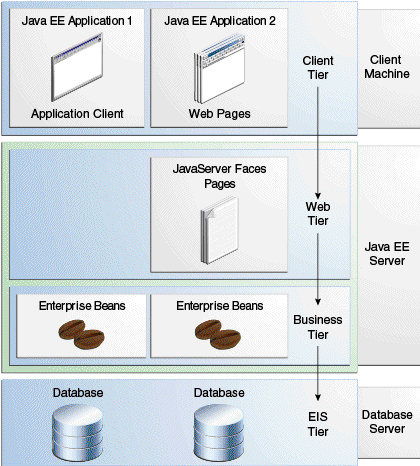
\includegraphics[resolution=150]{graphics/multitiered-application.png}
\caption{Architektura wielowarstwowa \autocite{jendrock2014jee}}
\end{figure}

Model ten jest powszechnie stosowany nie tylko dla aplikacji w Javie,
ale również przy użyciu wielu innych technologii.
\autocite{eisele2015modern, jendrock2014jee}

\subsection{JavaScript}\label{architektura---javascript}

Biorąc pod uwagę fakt, że JavaScript został stworzony do zastosowań w
aplikacjach klienckich, środowisko to nie posiada ustandaryzowanych
wzorców projektowania i tworzenia systemów informatycznych. Ze względu
na dużą i różnorodną społeczność wielu programistów o odmiennym podłożu
zawodowym, nieustannie powstaje szereg bibliotek oraz wiele modeli
aplikacyjnych, lecz jak dotąd nie wyłonił się z nich żaden dominujący
paradygmat. Jedynym wspólnym ich elementem jest Node.js, lecz biblioteka
ta nie dyktuje wzorców architektonicznych, poza posługiwaniem się
zdarzeniami i odwołaniami obsługi tychże.\\
Programowanie w JavaScript w dużej mierze opiera się na obsłudze
zdarzeń. Łatwo to zauważyć na przykładzie aplikacji przeglądarkowych,
gdzie zdarzenia są wywoływane przez interakcje użytkownika z
interfejsem, na przykład kliknięcia myszy czy przeciąganie obiektów. Z
perspektywy projektu języka, w JavaScript wprowadzono ułatwienia dla
programowania sterowanego zdarzeniami (ang. \emph{event-driven
programming}). Jednym z bardziej istotnych jest wprowadzenie funkcji
wyższego rzędu. Dzięki nim możliwe jest przekazywanie jako parametrów
funkcji innych funkcji jako odwołania do wykonanej akcji.

\begin{lstlisting}[numbers=left, caption=Obsługa zdarzeń kliknięcia]
function handleClick() {
    alert("Button clicked!");
};

var button = document.getElementById("button");
button.addEventListener("click", handleClick);
\end{lstlisting}

W linijce 6 powyższego listingu do obiektu button została dodana obsługa
zdarzenia. Jako pierwszy parametr metody \emph{addEventListener}
przekazano typ akcji - kliknięcie (\emph{`click'}) oraz drugi parametr
będący nazwą funkcji, która zostanie wykonana przy wykonaniu
zdefiniowanej akcji.

\subsubsection{libuv}\label{libuv}

libuv jest to natywna biblioteka stanowiącą warstwę abstrakcji nad
różnymi urządzeniami wejścia/wyjścia do wykonywania na nich
asynchronicznych operacji. Została zaprojektowana z myślą o Node.js,
lecz znalazła zastosowanie w innych projektach.\\
W skład jej możliwości wchodzą:

\begin{itemize}
\tightlist
\item
  asynchroniczna obsługa połączeń sieciowych poprzez TCP oraz UDP,
\item
  asynchroniczna obsługa plików oraz operacji na systemie plików,
\item
  zdarzenia systemu plików,
\item
  komunikacja między procesowa,
\item
  procesy pomne,
\item
  pula wątków,
\item
  obsługa przerwań,
\item
  zegar wysokiej rozdzielczości,
\item
  obsługa wątków i ich synchronizacja.
\end{itemize}

libuv udostępnia użytkownikom 2 interfejsy do pracy z wejściem/wyjściem:
uchwyt (ang. \emph{handle}) oraz zapytanie (ang. \emph{request}).\\
Uchwyty stanowią obiekty o długim czasie życia, zdolne do
przeprowadzania pewnych operacji w czasie aktywacji, przykładowo uchwyt
może implementować przyjmowanie połączeń na serwerze TCP i być
aktywowany za każdym razem gdy pojawia się nowe połączenie.\\
Zapytanie reprezentuje krótkotrwałe operacje, które mogą być wywoływane
samodzielnie lub w cyklu obsługi uchwytu. Powyższe abstrakcje służą
użytkownikom do interakcji z pętlą zdarzeń (ang. \emph{event loop}).\\
Pętla wejścia/wyjścia lub też pętla zdarzeń jest kluczową częścią libuv.
Odpowiada ona za przetwarzanie wszystkich operacji związanych z
wejściem/wyjściem, używając niecodziennego, jednowątkowego i
asynchronicznego modelu obsługi tychże operacji. Wszystkie działania
sieciowe wykonywane są w jednym wątku posługując się nieblokującymi
gniazdami (ang. \emph{socket}), które są cyklicznie odpytywane.\\
W przeciwieństwie do sieciowego wejścia/wyjścia, obsługa plików jest
bazowana na blokującym (synchronicznym) dostępie wykorzystującym pulę
wątków. Każdy wątek z puli może niezależnie przetwarzać operacje na
pliku.\\
Takie podejście do równoległości jest przykładem wzorca \emph{Reaktor}.

\subsubsection{Wzorzec Reaktor}\label{wzorzec-reaktor}

Wzorzec \emph{Reaktor} jest zaprojektowany do obsługi zapytań
przychodzących równolegle do systemu od jednego lub więcej klientów.
Każda funkcjonalność systemu jest reprezentowana przez osobne jednostki
przetwarzania odpowiedzialne za obsługę jedynie zapytań przeznaczonych
dla nich. Za podział zapytań pomiędzy jednostki przetwarzania
odpowiedzialny jest synchroniczny demultiplekser.\\
Kluczowymi elementami wzorca Reaktor są: uchwyty, demultiplekser zdarzeń
(ang. \emph{event demultiplexer}), dyspozytor wejściowy (ang.
\emph{initiation dispatcher}) oraz jednostki obsługi zdarzeń (ang.
\emph{event handler}).\\
Uchwyty są zasobami zarządzanymi przez system operacyjny. Wśród nich
znajdują się między innymi połączenia sieciowe czy otwarte pliki.\\
Synchroniczny demultiplekser zdarzeń blokuje nadchodzące zdarzenia w
oczekiwaniu na uchwyty i zwalnia blokadę kiedy operacja może zostać
przeprowadzona na uchwycie bez potrzeby blokowania.\\
Dyspozytor wejściowy definiuje interfejs do rejestracji, derejestracji i
dyspozycji jednostek obsługi zdarzeń. Jest on informowany o nowych
zdarzeniach w systemie, w wyniku czego wybiera odpowiednią jednostkę
obsługi zdarzenia do otrzymanej akcji.\\
Jednostka obsługi zdarzeń implementuje logikę przetwarzania
przychodzących zdarzeń. System rejestruje takie jednostki w dyspozytorze
wejściowym dla konkretnych typów zdarzeń. Kiedy jedno z nich zostanie
odebrane, dyspozytor rozwiązuje odpowiednią jednostkę obsługi zdarzeń i
wywołuje jej kod obsługi.

\begin{figure}[htbp]
\centering
\begingroup  \makeatletter  \providecommand\color[2][]{    \errmessage{(Inkscape) Color is used for the text in Inkscape, but the package 'color.sty' is not loaded}    \renewcommand\color[2][]{}  }  \providecommand\transparent[1]{    \errmessage{(Inkscape) Transparency is used (non-zero) for the text in Inkscape, but the package 'transparent.sty' is not loaded}    \renewcommand\transparent[1]{}  }  \providecommand\rotatebox[2]{#2}  \ifx\svgwidth\undefined    \setlength{\unitlength}{406.8bp}    \ifx\svgscale\undefined      \relax    \else      \setlength{\unitlength}{\unitlength * \real{\svgscale}}    \fi  \else    \setlength{\unitlength}{\svgwidth}  \fi  \global\let\svgwidth\undefined  \global\let\svgscale\undefined  \makeatother  \begin{picture}(1,0.44610383)    \put(0,0){\includegraphics[width=\unitlength,page=1]{handle-event.pdf}}    \put(0.0152409,0.40530717){\color[rgb]{0,0,0}\makebox(0,0)[lb]{\smash{Aplikacja}}}    \put(0,0){\includegraphics[width=\unitlength,page=2]{handle-event.pdf}}    \put(0.38987217,0.40530717){\color[rgb]{0,0,0}\makebox(0,0)[lb]{\smash{Dyspozytor}}}    \put(0,0){\includegraphics[width=\unitlength,page=3]{handle-event.pdf}}    \put(0.62881023,0.40530717){\color[rgb]{0,0,0}\makebox(0,0)[lb]{\smash{J. przetwarzania}}}    \put(0,0){\includegraphics[width=\unitlength,page=4]{handle-event.pdf}}    \put(0.88643068,0.40530717){\color[rgb]{0,0,0}\makebox(0,0)[lb]{\smash{Uchwyt}}}    \put(0,0){\includegraphics[width=\unitlength,page=5]{handle-event.pdf}}    \put(0.09685349,0.33181907){\color[rgb]{0,0,0}\makebox(0,0)[lb]{\smash{inicjalizuj Dyspozytora}}}    \put(0,0){\includegraphics[width=\unitlength,page=6]{handle-event.pdf}}    \put(0.09685349,0.27452743){\color[rgb]{0,0,0}\makebox(0,0)[lb]{\smash{zarejestruj J. przetwarzania}}}    \put(0,0){\includegraphics[width=\unitlength,page=7]{handle-event.pdf}}    \put(0.48033432,0.21723578){\color[rgb]{0,0,0}\makebox(0,0)[lb]{\smash{podaj uchwyt}}}    \put(0,0){\includegraphics[width=\unitlength,page=8]{handle-event.pdf}}    \put(0.08702065,0.15994413){\color[rgb]{0,0,0}\makebox(0,0)[lb]{\smash{obsłuż zdarzenie}}}    \put(0,0){\includegraphics[width=\unitlength,page=9]{handle-event.pdf}}    \put(0.49016716,0.10265249){\color[rgb]{0,0,0}\makebox(0,0)[lb]{\smash{wybierz}}}    \put(0,0){\includegraphics[width=\unitlength,page=10]{handle-event.pdf}}    \put(0.48033432,0.04536085){\color[rgb]{0,0,0}\makebox(0,0)[lb]{\smash{obsłuż zdarzenie}}}  \end{picture}\endgroup \caption{Sekwencja działania Reaktora (źródło: praca własna)}
\end{figure}

Po zarejestrowaniu wszystkich jednostek obsługi zdarzeń startowana jest
pętla obsługi zdarzeń (ang. \emph{event loop}) dyspozytora. Uchwyty
zostają powiązane z zarejestrowanymi z jednostkami obsługi, a
demultiplekser czeka na zdarzenia przychodzące na uchwytach. Po
nadejściu jednego z nich demultiplekser zawiadamia dyspozytora, że
uchwyt jest gotowy do rozpoczęcia przetwarzania danych. Ten z kolei,
używając typu źródła zdarzenia, wybiera jednostkę obsługi i wywołuje jej
kod.\\
Takie podejście pociąga za sobą szereg zalet jak i wad. Przede wszystkim
zapewnia łatwą kontrolę nad współbieżnością. Reaktor kolejkuje zdarzenia
na poziomie demultipleksowania i delegacji pracy do jednostek obsługi.
Jest to zwykle wystarczające, aby wyeliminować potrzebę stosowania
bardziej skomplikowanych metod synchronizacji i blokad w aplikacji.
Dodatkowo, wzorzec ten ułatwia rozdzielenie odpowiedzialności pomiędzy
komponenty systemu. Demultipleksowanie oraz delegacja jest niezależna od
aplikacji i może być reużywana w różnych projektach. Część funkcjonalna
systemu jest rozdzielona pomiędzy jednostki obsługi zdarzeń i każda z
nich jest odpowiedzialna za obsługę konkretnych typów zapytań.\\
Jednakże ceną przetwarzania jednowątkowego jest brak możliwości
wywłaszczenia wątku, jednostki obsługi zdarzeń wykonują pracę
nieprzerwanie. Z tego wynika, że żadne z nich nie powinno wykonywać
blokujących operacji, ponieważ w takim przypadku jeden zablokowałby cały
proces, ograniczając responsywność systemu. Co więcej, aplikacje
napisane z wykorzystaniem wzorca Rektor mogą być trudniejsze do analizy
i rozwiązywania błędów, ze względu na odwrócony proces przepływu
sterowania. Implementacja tego wzorca jest ograniczona do możliwości
systemu operacyjnego, który musi wspierać nieblokujące operacje. Ten
problem można obejść wykorzystując wiele wątków, w których przetwarzanie
odbywa się w sposób blokujący, jednak wyzbywając się korzyści
wynikających z braku przełączania
kontekstu.\autocite{schmidt1995reactor}

\subsection{Elixir}\label{architektura---elixir}

Erlang, a zatem i Elixir, to nie tylko języki programowania, ale również
zestaw narzędzi i wzorców programistycznych zwanych \emph{Open Telecom
Platform} (OTP).

\subsubsection{Open Telecom Platform}\label{open-telecom-platform}

Mimo swojej nazwy, OTP jest zbiorem bibliotek ogólnego zastosowania,
wprowadzający standardowe rozwiązania dla powszechnych problemów.
Dodatkowo zawiera narzędzia do rozproszonej komunikacji, wykrywania
błędów czy przeładowywania kodu działającego systemu. OTP wprowadza
struktury generyczne dla różnych projektów informatycznych, które mają
ułatwić pracę programistom, przykładowo ustandaryzowanej struktury
plików projektowych, standardową bibliotekę powszechnie stosowanych
funkcjonalności oraz zbiór tzw. \emph{behaviour} (ang.
\emph{zachowanie}) będących wzorcami projektowymi dla różnorodnych
systemów. Dzięki temu nowy pracownik zespołu może rozpoznać znane
wzorce, co ułatwia zapoznanie się z istniejącą bazą kodu.\\
Podejście do współbieżności w Erlangu/OTP znacznie różni się od
powszechnie stosowanego modelu dzielonej pamięci z blokadami. W tym
przypadku wykorzystywane są lekkie procesy, projektowane na \emph{model
aktorowy}, zarządzane przez wirtualną maszynę. Procesy te są od siebie
całkowicie odizolowane, nie jest wykorzystana dzielona pamięć. Ze
względu na taką separacje, komunikacja pomiędzy procesami odbywa się
poprzez przekazywanie wiadomości między sobą (ang. \emph{message
passing}). Dzielone informacje są kopiowane i przesyłane do innego
procesu. Dzięki temu nie jest możliwa wielodostępowa modyfikacja danych,
co zapobiega powstawaniu anomalii. Jednakże takie podejście nie jest bez
wad, gdyż powielanie dużych bloków pamięci może być kosztowne. W celu
zapewnienia wysokiej niezawodności i odporności na błędy wprowadzone
zostało jedno z ważniejszych \emph{zachowań} OTP, \emph{Supervisor}
(ang. \emph{nadzorca}). Jest on odpowiedzialny za tworzenie i
monitorowanie stanu procesów wykonawczych. W sytuacji gdy proces
wykonawczy, w wyniku błędu, przerwie pracę, wtedy nadzorca jest w stanie
przywrócić poprawne funkcjonowanie systemu odtwarzając wykonawcę w
normalnym stanie. Nadzorcy, będąc jedynie typem zachowania, mogą być
traktowani jako zwykłe procesy wykonawcze, a zatem ich stan może być
monitorowany przez innego nadzorcę tworząc w drzewa nadzorcze. W ten
sposób system nie posiada jednego punktu odpowiedzialnego za stabilność,
a jest on podzielony na sekcje.\\
Równie ważnym elementem OTP jest protokół komunikacji rozproszonej
Erlanga. Podobnie jak lekkie procesy wirtualnej maszyny, komunikacja
rozproszona bazuje na modelu aktorowym. Poza izolacją procesów na
różnych węzłach komunikacji, istotną cechą protokołu jest jego
transparentność. Wymiana wiadomości odbywa się w taki sam sposób jak
pomiędzy procesami na jednej maszynie. Każdy z rozproszonych węzłów jest
świadomy istnienia innych węzłów i może się z nimi komunikować tak jakby
tworzyły jeden spójny system.\autocite{logan2010erlang}

\begin{figure}[htbp]
\centering
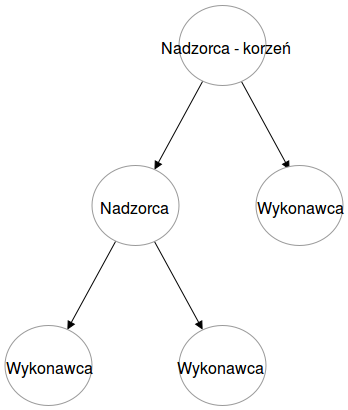
\includegraphics[resolution=130]{graphics/supervision-tree.png}
\caption{Schemat drzewa nadzorczego}
\end{figure}

\subsubsection{Model aktorowy}\label{model-aktorowy}

Model aktorowy jest modelem programowania, w którym przetwarzanie jest
wykonywane z natury współbieżnie. Podstawową jednostką wykonawczą tego
modelu jest \emph{aktor}.

Aktor jest jednostką wykonawczą, która odwzorowuje każdą przychodzącą
wiadomość na krotkę składającą się z:

\begin{itemize}
\tightlist
\item
  skończonego zbioru komunikatów przesłanych do innego aktora;
\item
  nowego zachowania, które wpłynie na odpowiedź następnego
  przetwarzanego komunikatu;
\item
  skończonego zbioru nowo utworzonych aktorów.
\end{itemize}

\begin{figure}[htbp]
\centering
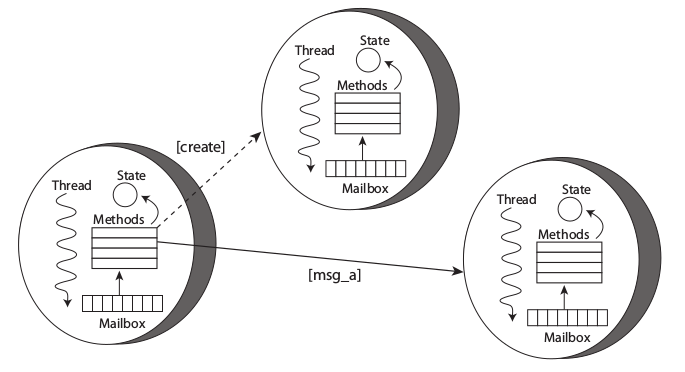
\includegraphics[resolution=130]{graphics/actor-messages.png}
\caption{Akcje w modelu aktorowym \autocite{karmani2009actor}}
\end{figure}

Aktorzy, w odróżnieniu od modelu współdzielonych zmiennych, nie dzielą
między sobą wspólnych obszarów pamięci. Informacje w obliczeniach
aktorów mogą być przekazywane, tylko i wyłącznie, poprzez wiadomości.
Model ze współdzieloną pamięcią nie dostarcza żadnych mechanizmów
abstrakcji i ukrywania informacji. Aby stwierdzić czy inny obiekt
otrzymał dostęp lub zmodyfikował wykorzystywane zmienne wymagane jest
zdefiniowanie odpowiedniego protokołu. Co więcej, nie można stwierdzić
czy na danych nie zostały wykonane niewłaściwe lub wręcz niepożądane
operacje. Jednym ze sposobów radzenia sobie z sytuacjami tego typu jest
wykorzystywanie blokad i synchronizacji. Model aktorowy zakłada, że
komunikacja pomiędzy aktorami nie jest synchroniczna, a akcje stanowią
częściowy porządek. Nadchodzące wiadomości trafiają do skrzynki
odbiorczej, gdzie czekają na przetworzenie. Wszystko to ma służyć
zapobieganiu blokowania i przetrzymywania zasobów, co może doprowadzić
do zakleszczeń (ang. \emph{deadlock}). Podstawową informacją zawartą w
wiadomości jest istnienie innego \emph{aktora}. Jest to spowodowane tym,
że \emph{aktor} A może skomunikować się z \emph{aktorem} B jedynie
znając jego \emph{nazwę}. Tę wiedzę może posiąść jeśli otrzymał ją w
chwili powstania lub poznał w wyniku przetwarzania nadchodzących
wiadomości. Co więcej, komunikacja jest transparentna. Pomimo
``świadomości'' istnienia innego aktora, nie jest znane jego położenie.
Umożliwia to utworzenie systemu aktorów fizycznie rozproszonych pomiędzy
wiele maszyn połączonych w sieć oraz dynamiczną rekonfigurację
topologii.\autocite{karmani2009actor, hewitt1977laws, agha86actors}

\subsection{Dyskusja}\label{dyskusja}

Poprzez wiele lat rozwoju i kolejne aktualizacje liczba standardów
zawartych w pakiecie Java Enterprise Edition zwiększyła się z 10 do 34.
Serwery aplikacyjne, które są podstawowym składnikiem budulcowym
aplikacji napisanych wykorzystujących Javę EE, dążą do pełnej
implementacji standardowej specyfikacji oraz wzbogacają ją o własne
rozwiązania. Niewiele z tych technologii wprowadza korzystne dla
architektury mikroserwisowej rozwiązania. Standard Java EE nigdy nie był
projektowany z myślą o systemach rozproszonych, poza wydzieleniem
warstwy bazodanowej i klienckiej. W związku z powyższym, na starcie
utrzymujemy w systemie dużą bazę kodu, który nie zostanie wykorzystany.
Stosowanie serwerów aplikacyjnych zakłada wdrażanie na jednym z nich
wielu usług jednocześnie. Biorąc po uwagę fakt, że taki serwer pracuje w
jednym procesie wirtualnej maszyny Javy, aplikacje działające pod jego
nadzorem mogą zakłócać działanie sobie nawzajem, a w najgorszym
przypadku jedna z nich może doprowadzić do awarii wszystkich poprzez
przerwanie działania samego serwera.

Tworzenie aplikacji monolitycznych jest możliwe przy wykorzystaniu
Node.js, lecz zastosowanie jednowątkowego wzorca Rektor nie sprzyja
takiemu podejściu. Z tego względu lepszym rozwiązaniem wydaje się
wydzielenie poszczególnych funkcjonalności na osobne programy, dzięki
czemu mogą wykorzystać zasoby systemów wieloprocesorowych bez wzajemnej
ingerencji w działanie. Z tego powodu, pomimo braku standardowych
rozwiązań, zastosowanie architektury mikroserwisowej jest popularnym
wyborem w środowisku JavaScript i wokół tego modelu rozwijanych jest
szereg narzędzi i bibliotek.

Podobnie ja w przypadku języka JavaScript, w Elixirze nie istnieją
standardowe wzorce architektoniczne systemów informatycznych. OTP
sugeruje jedynie kształt podstawowych elementów budulcowych aplikacji,
nie narzucając projektu. Monolityczne oprogramowanie stworzone w
Elixirze można podzielić na mniejsze usługi wydzielając niezależne grupy
procesów (aktorów) jako działające niezależne programy. Do komunikacji
między procesami w architekturze mikroserwisowej popularnym wyborem jest
HTTP. Jednakże, przy użyciu Elixira, usługi mogą porozumiewać się przy
pomocy protokołu rozproszonej komunikacji wirtualnej maszyny Erlanga.
Jest to także ułatwienie dla programistów, gdyż wykorzystanie jego jest
transparentne z punktu widzenia użytkownika.{[}patrz
\ref{skalowalnoux15bux107}{]} OTP ze względu na pochodzenie ze
środowiska Erlanga jest technologią dojrzałą, stabilną oraz aktywnie
rozwijaną przez społeczność Elixira. \autocite{valim2015microservices}
\clearpage{}
	\clearpage{}\section{Wydajność}\label{wydajnoux15bux107}

Wydajność technologii można mierzyć na wielu płaszczyznach, a na
otrzymane wyniki wpływa duża liczba czynników. Przedstawiane środowiska
programistyczne zostały przetestowane pod kątem wydajności, w kilku
odmiennych scenariuszach.

Wybrano 4 przypadki w 3 kategoriach:

\begin{itemize}
\tightlist
\item
  Duża liczba zapytań:

  \begin{itemize}
  \tightlist
  \item
    zapytania nie wymagające dużej mocy obliczeniowej
  \end{itemize}
\item
  Czasochłonne obliczenia:

  \begin{itemize}
  \tightlist
  \item
    obliczenia na liczbach całkowitych
  \item
    operacje macierzowe
  \end{itemize}
\item
  Ograniczenia wejścia/wyjścia

  \begin{itemize}
  \tightlist
  \item
    operacje na systemie plików
  \end{itemize}
\end{itemize}

Wyżej wymienione sytuacje są powszechnie spotykane w współczesnych
systemach informatycznych.

Badania przeprowadzono na sprzęcie o następujących parametrach:

Maszyna testowa:

\begin{itemize}
\tightlist
\item
  Procesor: Intel(R) Core(TM)2 Duo CPU L9400 @ 1.86GHz
\item
  Pamięć: 4GB DDR2 800MHz
\item
  System operacyjny: GNU/Linux 4.2.5-1-ARCH
\end{itemize}

Maszyna testująca:

\begin{itemize}
\tightlist
\item
  Procesor: Intel(R) Core(TM)2 Quad CPU Q9550 @ 2.83GHz
\item
  Pamięć: 4GB DDR2 800MHz
\item
  System operacyjny: GNU/Linux 4.2.5-1-ARCH
\end{itemize}

Na maszynę testującą celowo wybrano komputer o większej mocy, aby
zapewnić ciągłość testów i uniknąć komplikacji wynikających z
niewystarczającej mocy do analizy danych. Komputery podłączono
bezpośrednio w sieć o przepustowości 1Gb/s.\\
Oprogramowanie wykorzystane do implementacji oraz przeprowadzenia testów
wybrano na podstawie powszechności zastosowania. Parametr ten określono
w oparciu statystyki dostępne w publicznych repozytoriach
\autocite{npm2015,mavenrepo2015, hex2015}.\\
Rozwiązanie w języku Java stworzono na bazie serwera aplikacyjnego
WildFly, będącego otwartą dla społeczności dystrybucją serwera JBoss
Enterprise Application Platform firmy RedHat. Wspiera on najnowszą
dostępną wersję standardu Java EE 7.\\
W implementacji kodu JavaScript i Node.js wykorzystano bibliotekę
Express.js udostępniającą podstawowe mechanizmy wymagane do stworzenia
aplikacji internetowej, przy zapewnieniu stabilności dla rozwiązań
produkcyjnych. Rozwiązanie w języku Elixir korzysta z pakietu Phoenix
Framework, gromadzącego dojrzałe technologie, przeznaczone do zastosowań
w usługach internetowych.\\
Do przeprowadzenia badań wykorzystano oprogramowanie Gatling. Udostępnia
ono, bazujący na języku Scala, język definiowania testów obciążeniowych.

Wersje oprogramowania:

\begin{itemize}
\tightlist
\item
  Java: 1.8.0\_66
\item
  Wildfly: 9.0.1.Final
\item
  Node.js: v5.3.0
\item
  Express.js: 4.13.1
\item
  Elixir: 1.1.1
\item
  Phoenix Framework: 1.0.3
\item
  Scala: 2.11.7
\item
  Gatling: 2.1.7
\end{itemize}

\subsection{Duża liczba zapytań}\label{duux17ca-liczba-zapytaux144}

Wiele aplikacji używanych na co dzień korzysta z łączności sieciowej.
Obserwuje się w ostatnich latach znaczny wzrost na rynku usług zdalnych,
a także zwiększenie liczby użytkowników owych usług. Z tego względu
współczesne systemy informatyczne muszą być w stanie obsłużyć znaczną
liczbę jednoczesnych połączeń i zapytań.

Test polega na wykonaniu metody HTTP GET na serwerze zwracającym prosty
łańcuch tekstowy. Zasymulowano 350000 użytkowników wykonujących żądanie
niezależnie, rozłożonych na przestrzeni 100 sekund.

Implementacje we wszystkich trzech technologiach są trywialne, polegają
na prostym umieszczeniu łańcucha znaków w odpowiedzi, więc zostały
pominięte.

\subsubsection{Java}\label{java}

\begin{figure}[htbp]
\centering
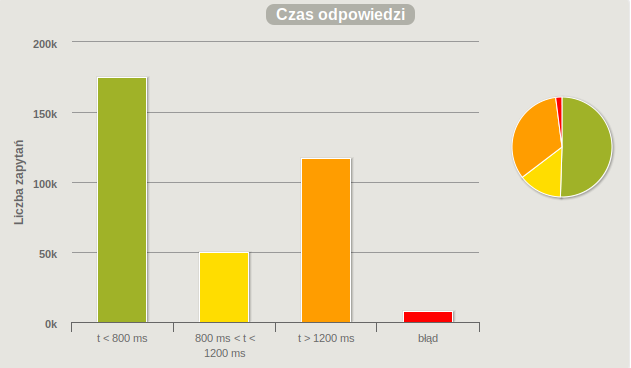
\includegraphics[resolution=150]{test_results/java/simpletest/screenshots/response_times.png}
\caption{Wykres czasu odpowiedzi na zapytania (źródło: praca własna)}
\end{figure}

Na połowę zapytań otrzymano odpowiedź w czasie poniżej 800 milisekund, a
nieznaczna cześć z nich została oznaczona jako błędne.

\begin{figure}[htbp]
\centering
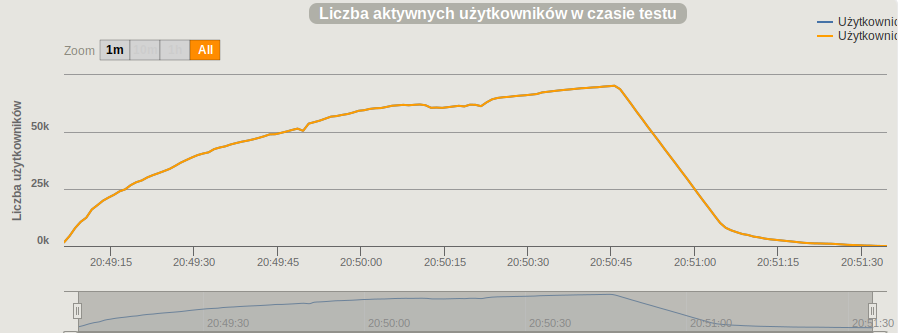
\includegraphics[resolution=150]{test_results/java/simpletest/screenshots/active_users.png}
\caption{Wykres aktywnych użytkowników w czasie trwania testu (źródło: praca własna)}
\end{figure}

\emph{Liczba aktywnych użytkowników} przedstawia zapytania oczekujące na
odpowiedź w danej chwili czasu. Liczba aktywnych użytkowników rośnie w
przybliżeniu jednostajnie. Odpowiedź na ostatnie żądanie użytkownik
otrzymał po 30 sekundach od jego wysłania.

\begin{figure}[htbp]
\centering
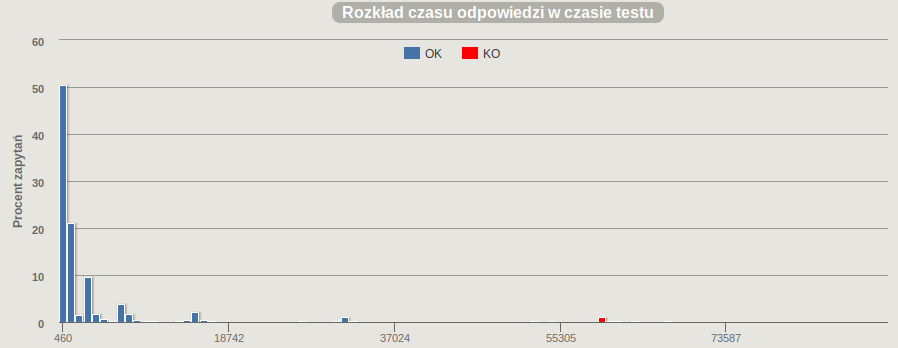
\includegraphics[resolution=150]{test_results/java/simpletest/screenshots/distribution.png}
\caption{Wykres rozkładu czasu odpowiedzi w czasie testu (źródło: praca własna)}
\end{figure}

Większość czasów odpowiedzi plasuje się na lewym krańcu wykresu.
Występują pojedyncze wyjątki, niewielka część przekroczyła maksymalny
czas oczekiwania 60 sekund.

\begin{figure}[htbp]
\centering
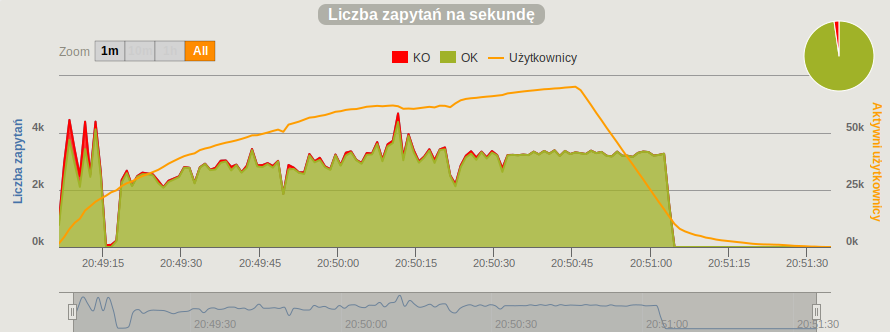
\includegraphics[resolution=150]{test_results/java/simpletest/screenshots/requests.png}
\caption{Wykres liczby zapytań na sekundę w czasie testu (źródło: praca własna)}
\label{java:simple:requests}
\end{figure}

Wirtualna maszyna Javy potrzebuje czasu na, tak zwane, \emph{rozgrzanie
się}. Wtedy dokonuje wczytania niezbędnych komponentów i automatycznej
optymalizacji kodu bajtowego. Zjawisko to można zaobserwować na wykresie
\ref{java:simple:requests}. Na początku testu wiele żądań zostało
oznaczonych jako błędnych, lecz po dokonaniu poprawek przez maszynę
wirtualną liczba przyjmowanych zapytań na sekundę ustabilizowała się.

\begin{figure}[htbp]
\centering
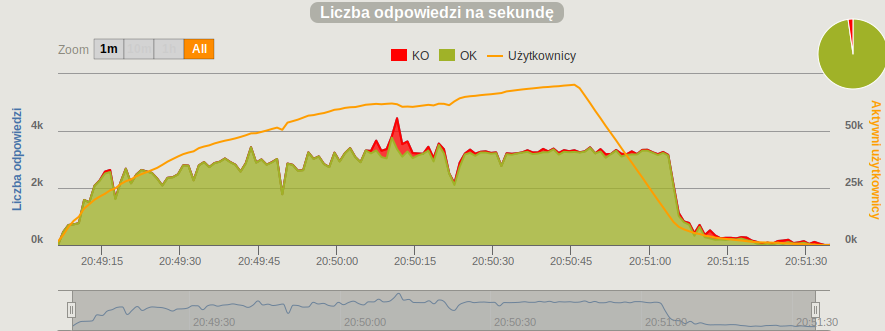
\includegraphics[resolution=150]{test_results/java/simpletest/screenshots/responses.png}
\caption{Wykres liczby odpowiedzi na sekundę w czasie trwania testu (źródło: praca własna)}
\label{java:simple:responses}
\end{figure}

Wykres \ref{java:simple:responses} również odzwierciedla proces
optymalizacji. W granicy 60 sekundy testu zauważono zwiększoną liczbę
błędnych odpowiedzi. Część zapytań przyjętych przed optymalizacją nie
została poprawnie przetworzona.

\begin{figure}[htbp]
\centering
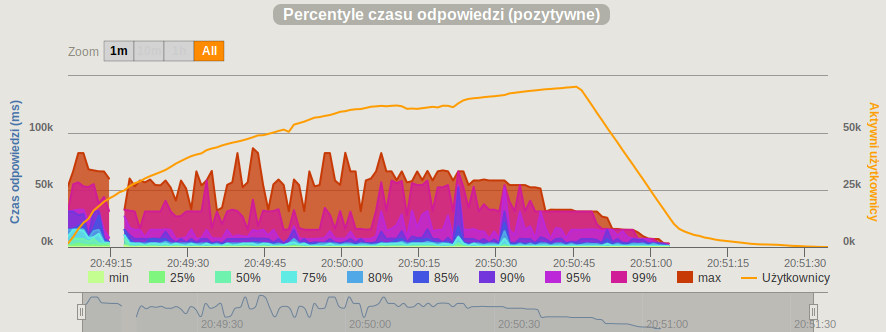
\includegraphics[resolution=150]{test_results/java/simpletest/screenshots/response_percentile.png}
\caption{Wykres percentyli czasu odpowiedzi w czasie trwania testu (źródło: praca własna)}
\label{java:simple:response_percentile}
\end{figure}

\begin{figure}[htbp]
\centering
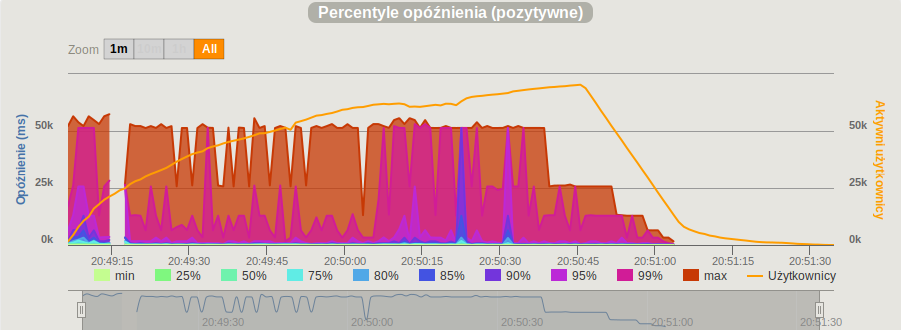
\includegraphics[resolution=150]{test_results/java/simpletest/screenshots/latency_percentile.png}
\caption{Wykres percentyli opóźnienia w czasie trwania testu (źródło: praca własna)}
\label{java:simple:latency_percentile}
\end{figure}

Rysunki
\ref{java:simple:response_percentile},\ref{java:simple:latency_percentile}
przedstawiają dane jedynie dla poprawnie przetworzonych zapytań.
\emph{Czas odpowiedzi} jest różnicą czasu otrzymania pełnej odpowiedzi
od czasu wysłania zapytania. \emph{Opóźnienie} stanowi czas, który
upłynął od wysłania zapytania do otrzymania pierwszego bajta odpowiedzi.
W granicach 20:50:10 zauważono zmianę zarówno w czasie odpowiedzi jak i
opóźnieniu. Została ona poprzedzona utratą części przetwarzanych
zapytań, wywołaną uruchomieniem odśmiecacza pamięci (ang. \emph{garbage
collector}). Po tym zabiegu czasy poprawiły się i zostały
zakwalifikowane do niższej kategorii na wykresach percentyli.

\begin{longtable}[c]{@{}llll@{}}
\caption{Statystyki Java w teście prostego zapytania}\tabularnewline
\toprule
& W sumie & OK & KO\tabularnewline
\midrule
\endfirsthead
\toprule
& W sumie & OK & KO\tabularnewline
\midrule
\endhead
Zapytania & 350000 & 342147 & 7853\tabularnewline
Średnia l./s & 2361,052 & 2308,077 & 52,975\tabularnewline
& & &\tabularnewline
Min & 3 & 3 & 9\tabularnewline
50 percentyl & 602 & 337 & 60032\tabularnewline
75 percentyl & 3026 & 3019 & 61503\tabularnewline
95 percentyl & 25211 & 15071 & 67298\tabularnewline
99 percentyl & 61040 & 32740 & 91059\tabularnewline
Max & 91412 & 86686 & 91412\tabularnewline
Średnia & 4155 & 2894 & 59091\tabularnewline
Odchylenie standardowe & 11121 & 7160 & 13856\tabularnewline
\bottomrule
\end{longtable}

\subsubsection{JavaScript}\label{javascript}

\begin{figure}[htbp]
\centering
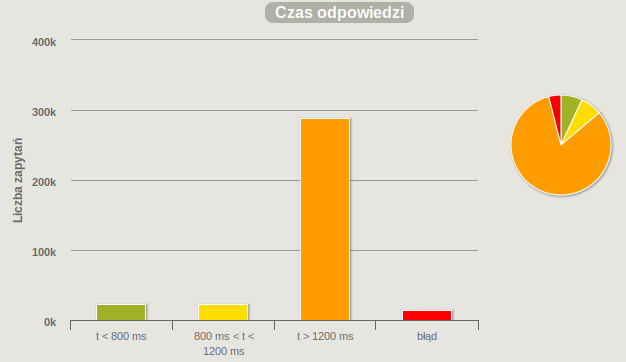
\includegraphics[resolution=150]{test_results/js/simpletest/screenshots/response_times.png}
\caption{Wykres czasu odpowiedzi na zapytania (źródło: praca własna)}
\end{figure}

83\% zapytań zostało obsłużonych w czasie większym niż 1200 milisekund
oraz 4\% z całości oznaczono jako błędne.

\begin{figure}[htbp]
\centering
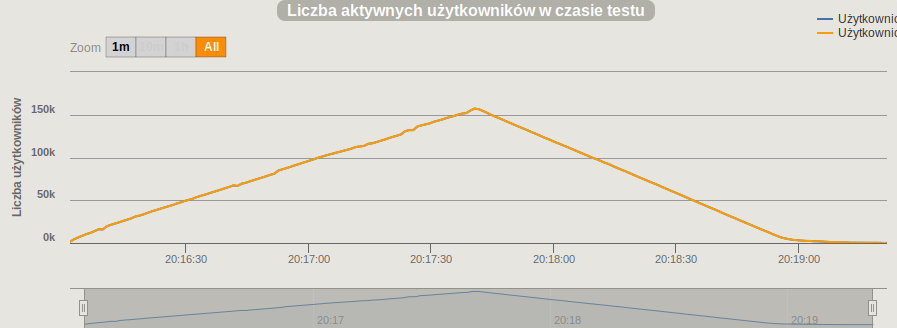
\includegraphics[resolution=150]{test_results/js/simpletest/screenshots/active_users.png}
\caption{Wykres aktywnych użytkowników w całym czasie trwania testu (źródło: praca własna)}
\end{figure}

Liczba aktywnych użytkowników rośnie liniowo i po otrzymaniu ostatniego
żądania również liniowo spada obsługując oczekujących użytkowników.

\begin{figure}[htbp]
\centering
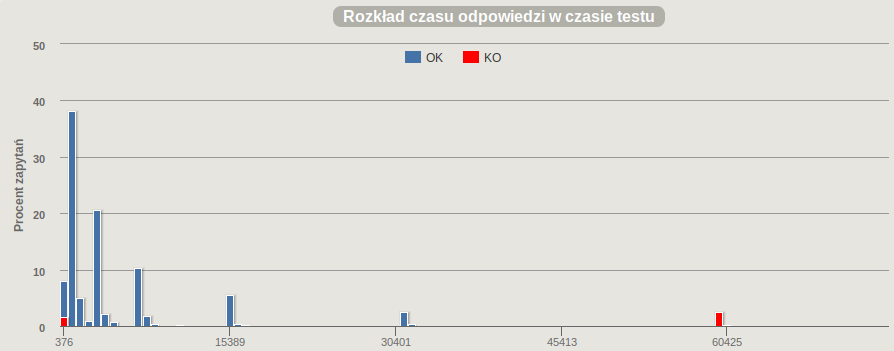
\includegraphics[resolution=150]{test_results/js/simpletest/screenshots/distribution.png}
\caption{Wykres rozkładu czasu odpowiedzi w czasie testu (źródło: praca własna)}
\end{figure}

\begin{figure}[htbp]
\centering
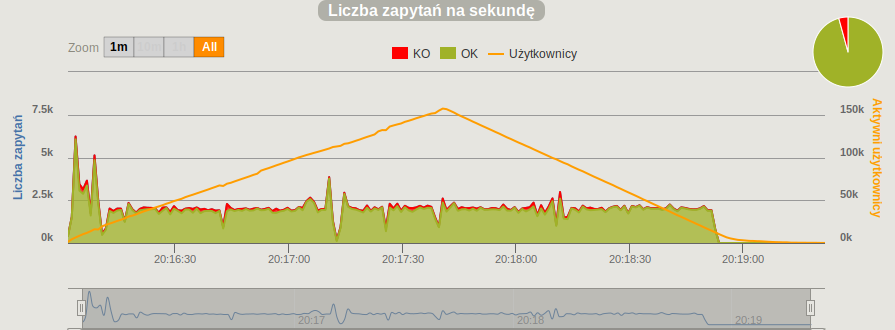
\includegraphics[resolution=150]{test_results/js/simpletest/screenshots/requests.png}
\caption{Wykres liczby zapytań na sekundę w czasie testu (źródło: praca własna)}
\end{figure}

Liczba przyjmowanych zapytań na sekundę utrzymuje stały poziom w czasie
trwania testu. Zauważono małe zaburzenia stanowiące nieznaczną część
całości testu.

\begin{figure}[htbp]
\centering
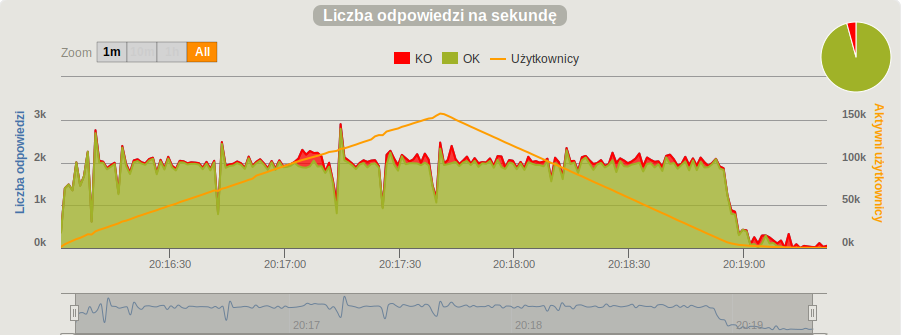
\includegraphics[resolution=150]{test_results/js/simpletest/screenshots/responses.png}
\caption{Wykres liczby odpowiedzi na sekundę w czasie trwania testu (źródło: praca własna)}
\end{figure}

Podobnie jak przyjmowanie, przetwarzanie i czas odpowiedzi na żądania
został utrzymany na stałym poziomie. Jednakże liczba zapytań
przekroczyła możliwości obsługi, w związku z czym po 60 sekundach
zauważono wzrost w ilości błędów.

\begin{figure}[htbp]
\centering
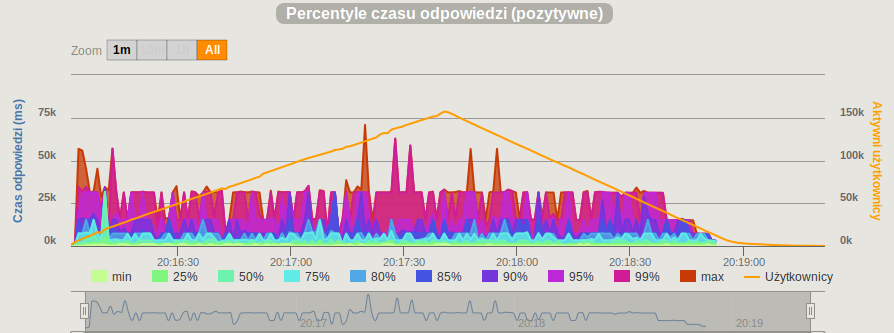
\includegraphics[resolution=150]{test_results/js/simpletest/screenshots/response_percentile.png}
\caption{Wykres percentyli czasu odpowiedzi w czasie trwania testu (źródło: praca własna)}
\end{figure}

Percentyle czasu odpowiedzi oraz opóźnienia utrzymują się na zbliżonym
poziomie w całym czasie trwania testu.

\begin{figure}[htbp]
\centering
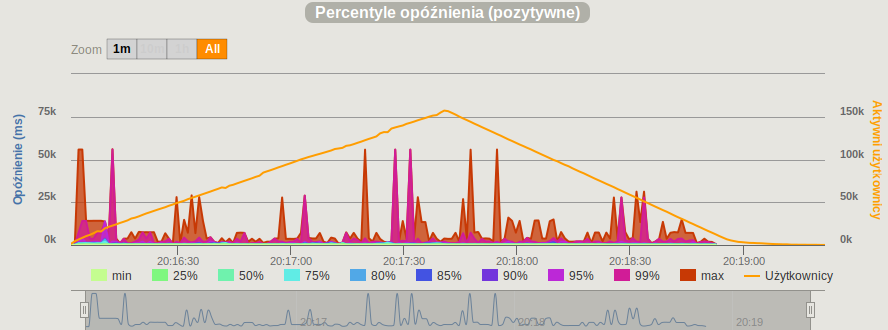
\includegraphics[resolution=150]{test_results/js/simpletest/screenshots/latency_percentile.png}
\caption{Wykres percentyli opóźnienia w czasie trwania testu (źródło: praca własna)}
\end{figure}

\begin{longtable}[c]{@{}llll@{}}
\caption{Statystyki JavaScript w teście prostego
zapytania}\tabularnewline
\toprule
& W sumie & OK & KO\tabularnewline
\midrule
\endfirsthead
\toprule
& W sumie & OK & KO\tabularnewline
\midrule
\endhead
Zapytania & 350000 & 335176 & 14824\tabularnewline
Średnia l./s & 1741,328 & 1667,575 & 73,753\tabularnewline
& & &\tabularnewline
Min & 1 & 1 & 8\tabularnewline
50 percentyl & 2039 & 1932 & 60006\tabularnewline
75 percentyl & 4826 & 4011 & 60011\tabularnewline
95 percentyl & 31244 & 15422 & 60041\tabularnewline
99 percentyl & 60012 & 31353 & 60613\tabularnewline
Max & 75062 & 70845 & 75062\tabularnewline
Średnia & 5847 & 4462 & 37180\tabularnewline
Odchylenie standardowe & 10805 & 6237 & 29181\tabularnewline
\bottomrule
\end{longtable}

\clearpage

\subsubsection{Elixir}\label{elixir}

\begin{figure}[htbp]
\centering
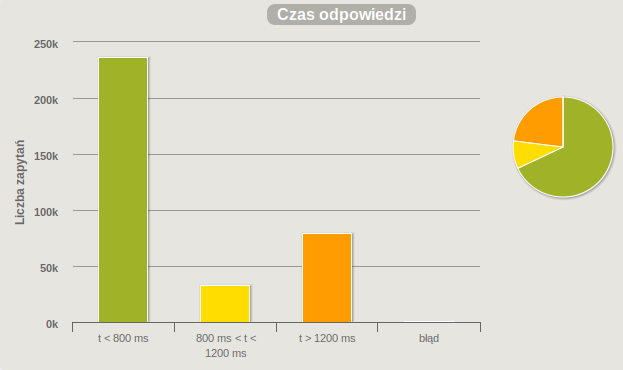
\includegraphics[resolution=150]{test_results/elixir/simpletest/screenshots/response_times.png}
\caption{Wykres czasu odpowiedzi na zapytania (źródło: praca własna)}
\end{figure}

Spośród wszystkich zapytań, na 93\% otrzymano odpowiedzi w czasie
mniejszym niż 800ms oraz nie wykazano żadnych błędów.

\begin{figure}[htbp]
\centering
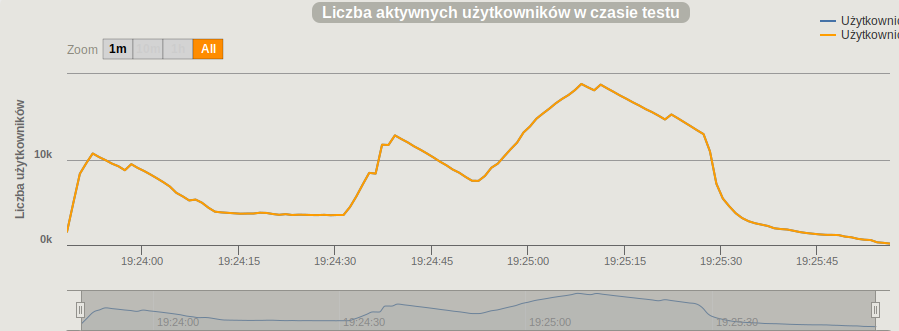
\includegraphics[resolution=150]{test_results/elixir/simpletest/screenshots/active_users.png}
\caption{Wykres aktywnych użytkowników w czasie trwania testu (źródło: praca własna)}
\end{figure}

Liczba aktywnych użytkowników stabilizuje się po 25 sekundach od
rozpoczęcia testu.

\begin{figure}[htbp]
\centering
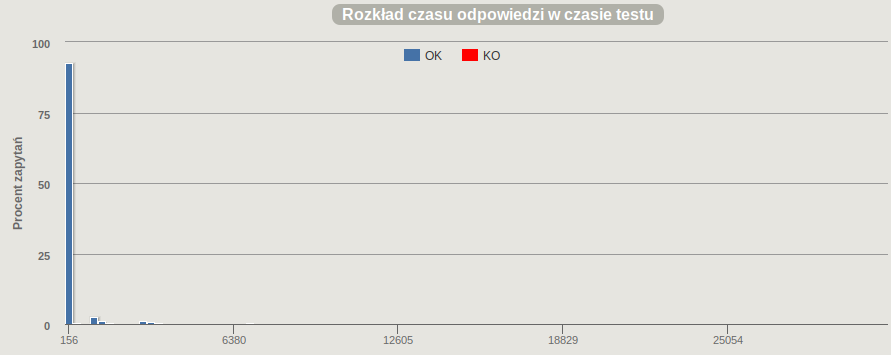
\includegraphics[resolution=150]{test_results/elixir/simpletest/screenshots/distribution.png}
\caption{Wykres rozkładu czasu odpowiedzi w czasie testu (źródło: praca własna)}
\end{figure}

\begin{figure}[htbp]
\centering
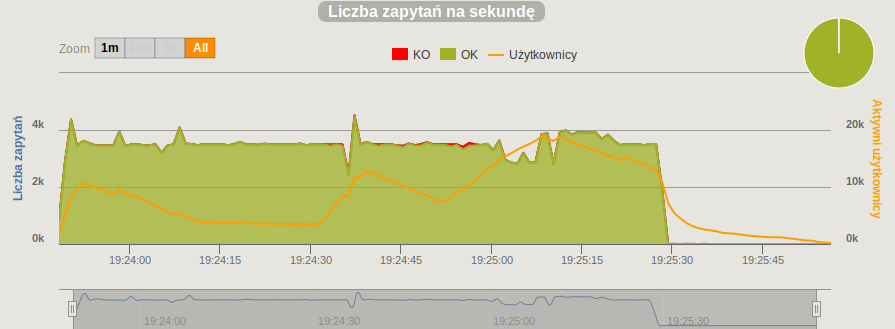
\includegraphics[resolution=150]{test_results/elixir/simpletest/screenshots/requests.png}
\caption{Wykres liczby zapytań na sekundę w czasie testu (źródło: praca własna)}
\end{figure}

Na wykresach \ref{elixir:simple:response_percentile} oraz
\ref{elixir:simple:latency_percentile} wyraźnie widać czas stabilizacji
aplikacji, po którym aplikacja zaczęła przyjmować zapytania na stałym
poziomie.

\begin{figure}[htbp]
\centering
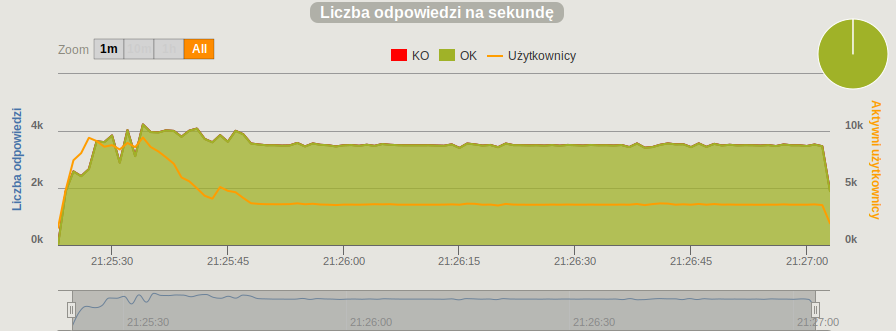
\includegraphics[resolution=150]{test_results/elixir/simpletest/screenshots/responses.png}
\caption{Wykres liczby odpowiedzi na sekundę w czasie trwania testu (źródło: praca własna)}
\end{figure}

Wykres liczby odpowiedzi odpowiada wykresowi liczby zapytań, stała
liczba odpowiedzi na sekundę i brak błędów.

\begin{figure}[htbp]
\centering
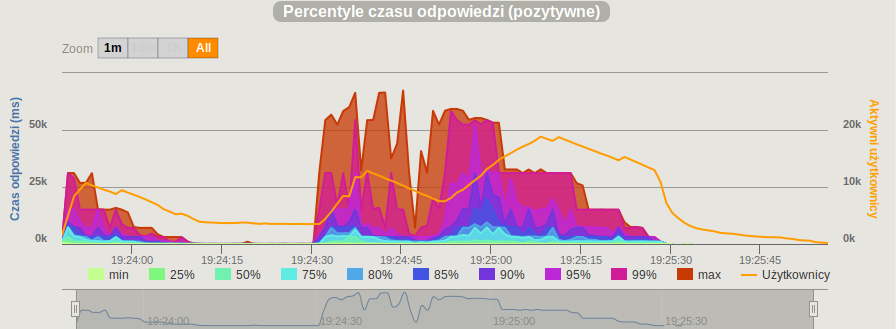
\includegraphics[resolution=150]{test_results/elixir/simpletest/screenshots/response_percentile.png}
\caption{Wykres percentyli czasu odpowiedzi w czasie trwania testu (źródło: praca własna)}
\label{elixir:simple:response_percentile}
\end{figure}

\begin{figure}[htbp]
\centering
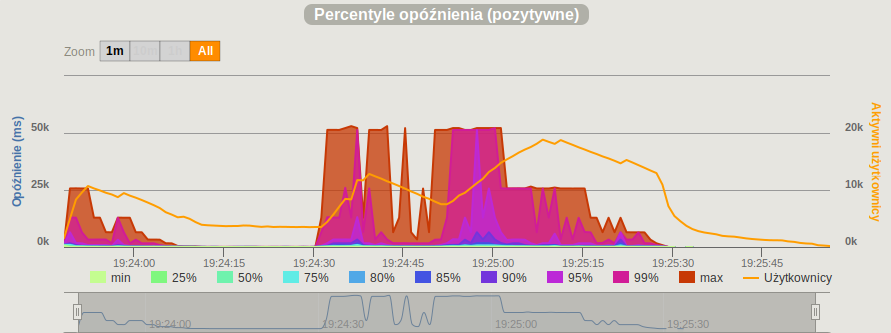
\includegraphics[resolution=150]{test_results/elixir/simpletest/screenshots/latency_percentile.png}
\caption{Wykres percentyli opóźnienia w czasie trwania testu (źródło: praca własna)}
\label{elixir:simple:latency_percentile}
\end{figure}

\begin{longtable}[c]{@{}llll@{}}
\caption{Statystyki Elixir w teście prostego zapytania}\tabularnewline
\toprule
& W sumie & OK & KO\tabularnewline
\midrule
\endfirsthead
\toprule
& W sumie & OK & KO\tabularnewline
\midrule
\endhead
Zapytania & 350000 & 350000 & 0\tabularnewline
Średnia l./s & 3498.74 & 3498.74 & -\tabularnewline
& & &\tabularnewline
Min & 0 & 0 & -\tabularnewline
50 percentyl & 9 & 9 & -\tabularnewline
75 percentyl & 26 & 26 & -\tabularnewline
95 percentyl & 1071 & 1071 & -\tabularnewline
99 percentyl & 4270 & 4270 & -\tabularnewline
Max & 31123 & 31123 & -\tabularnewline
Średnia & 223 & 223 & -\tabularnewline
Odchylenie standardowe & 1107 & 1107 & -\tabularnewline
\bottomrule
\end{longtable}

\clearpage

\subsection{Czasochłonne obliczenia}\label{czasochux142onne-obliczenia}

Współczesne systemy informatyczne wykonują wiele skomplikowanych
operacji. Ważna jest nie tylko możliwość obsługi dużej liczby zapytań,
ale także wykorzystanie mocy obliczeniowej sprzętu do wykonywania
operacji.\\
Celem tego testu jest sprawdzenie wydajności technologii przy
równoczesnym dostępnie wielu użytkowników, jednocześnie testując
wsparcie dla dużych liczb.

Test polega na wykonaniu metody HTTP GET na serwerze zwracającym 100000
element ciągu Fibonacciego. Zasymulowano 1000 użytkowników wykonujących
zapytanie niezależnie, rozłożonych na przestrzeni 100 sekund.

\subsubsection{Java}\label{java-1}

\begin{lstlisting}[language=Java, numbers=left, caption=Java - obliczanie n-tego elementu ciągu Fibonacciego]
import java.math.BigDecimal;

public class Fibonacci {
    public static BigDecimal calculateNth(long n) {
        BigDecimal result = new BigDecimal(n);
        if (n < 2) {
            return result;
        }

        BigDecimal n1 = new BigDecimal(0);
        BigDecimal n2 = new BigDecimal(1);
        n--;
        while (n > 0) {
            result = n1.add(n2);
            n1 = n2;
            n2 = result;
            n--;
        }

        return result;
    }
}
\end{lstlisting}

W implementacji zastosowano iteracyjny algorytm wyznaczania n-tego
elementu ciągu Fibonacciego. Wybrano tę wersję algorytmu ze względu na
możliwość wystąpienia przepełnienia stosu przy wykorzystaniu jej
rekurencyjnego odpowiednika. Do przechowywania dużych wartości
całkowitych wykorzystano klasę BigDecimal, należącą do standardowej
biblioteki Javy.

\begin{figure}[htbp]
\centering
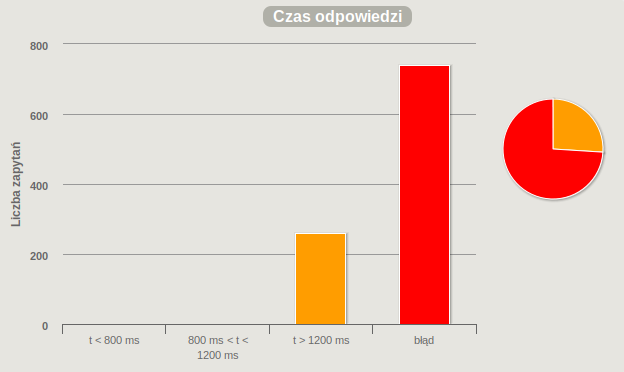
\includegraphics[resolution=150]{test_results/java/fibonacci/screenshots/response_times.png}
\caption{Wykres czasu odpowiedzi na zapytania (źródło: praca własna)}
\end{figure}

74\% zapytań zostało oznaczonych jako błędne z powodu przekroczenia
limitu oczekiwania wynoszącego 60 sekund.

\begin{figure}[htbp]
\centering
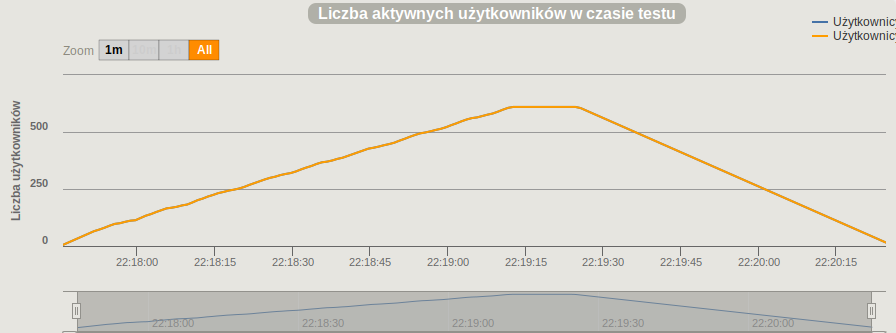
\includegraphics[resolution=150]{test_results/java/fibonacci/screenshots/active_users.png}
\caption{Wykres aktywnych użytkowników w czasie trwania testu (źródło: praca własna)}
\end{figure}

\begin{figure}[htbp]
\centering
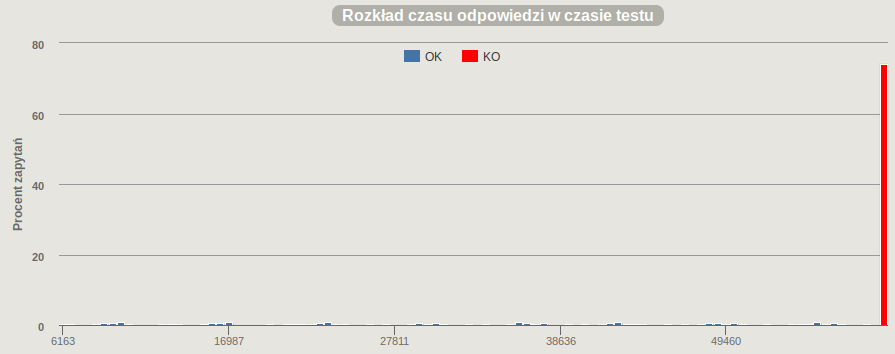
\includegraphics[resolution=150]{test_results/java/fibonacci/screenshots/distribution.png}
\caption{Wykres rozkładu czasu odpowiedzi w czasie testu (źródło: praca własna)}
\end{figure}

\begin{figure}[htbp]
\centering
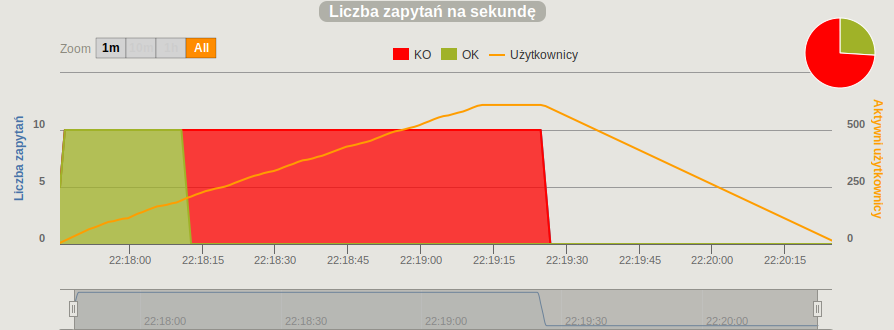
\includegraphics[resolution=150]{test_results/java/fibonacci/screenshots/requests.png}
\caption{Wykres liczby zapytań na sekundę w czasie testu (źródło: praca własna)}
\end{figure}

Po upłynięciu 1/3 testu serwer przestał przyjmować zapytania. Wynika to
z przyjętego modelu współbieżności. Nadchodzące zapytanie jest
obsługiwane w nowym wątku lub reużywany jest jeden z wcześniej
utworzonych wątków. Przy takim natężeniu wymagających czasowo żądań,
osiągnięto limit wykorzystywanych wątków. W związku z tym kolejne
nadchodzące zapytania nie mogły zostać przetworzone.

\begin{figure}[htbp]
\centering
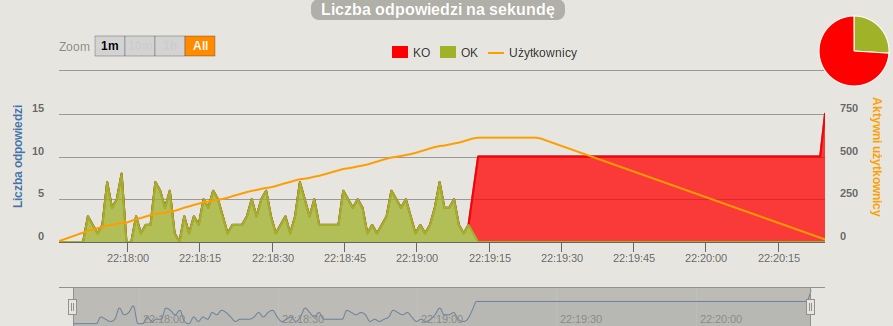
\includegraphics[resolution=150]{test_results/java/fibonacci/screenshots/responses.png}
\caption{Wykres liczby odpowiedzi na sekundę w czasie trwania testu (źródło: praca własna)}
\end{figure}

\begin{figure}[htbp]
\centering
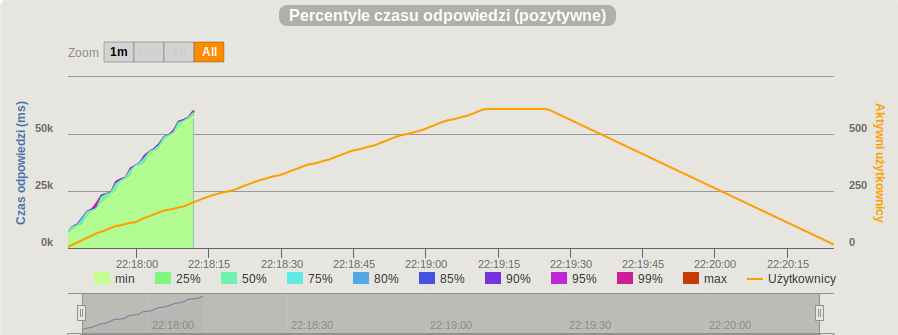
\includegraphics[resolution=150]{test_results/java/fibonacci/screenshots/response_percentile.png}
\caption{Wykres percentyli czasu odpowiedzi w czasie trwania testu (źródło: praca własna)}
\end{figure}

\begin{figure}[htbp]
\centering
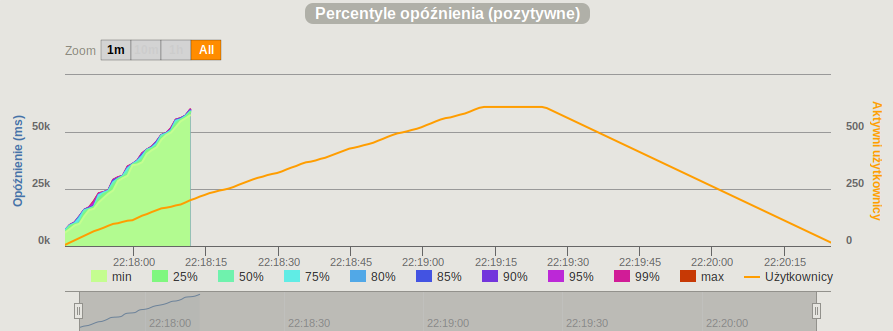
\includegraphics[resolution=150]{test_results/java/fibonacci/screenshots/latency_percentile.png}
\caption{Wykres percentyli opóźnienia w czasie trwania testu (źródło: praca własna)}
\end{figure}

\begin{longtable}[c]{@{}llll@{}}
\caption{Statystyki Java w teście z wykorzystaniem czasochłonnych
obliczeń}\tabularnewline
\toprule
& W sumie & OK & KO\tabularnewline
\midrule
\endfirsthead
\toprule
& W sumie & OK & KO\tabularnewline
\midrule
\endhead
Zapytania & 1000 & 260 & 740\tabularnewline
Średnia l./s & 6,253 & 1,626 & 4,627\tabularnewline
& & &\tabularnewline
Min & 5892 & 5892 & 60000\tabularnewline
50 percentyl & 60011 & 32751 & 60011\tabularnewline
75 percentyl & 60011 & 45996 & 60011\tabularnewline
95 percentyl & 60011 & 56091 & 60011\tabularnewline
99 percentyl & 60011 & 58727 & 60012\tabularnewline
Max & 60014 & 59941 & 60014\tabularnewline
Średnia & 52915 & 32721 & 60010\tabularnewline
Odchylenie standardowe & 14326 & 15440 & 1\tabularnewline
\bottomrule
\end{longtable}

\clearpage

\subsubsection{JavaScript}\label{javascript-1}

\begin{lstlisting}[numbers=left, caption=JavaScript - obliczanie n-tego elementu ciągu Fibonacciego]
var BigNum = require('bignum');

function calculateNth(n) {
    var result = BigNum(n);
    if (n < 2) {
        return result;
    }

    var n1 = BigNum(0);
    var n2 = BigNum(1);
    n -= 1;
    while (n > 0) {
        result = n1.add(n2);
        n1 = n2;
        n2 = result;
        n -= 1;
    }

    return result;
}
\end{lstlisting}

Powyższa implementacja jest translacją wersji w języku Java. JavaScript
nie posiada w standardzie wsparcia dla dużych liczb całkowitych. Do ich
przechowywania wykorzystano bibliotekę \emph{bignum}.

\begin{figure}[htbp]
\centering
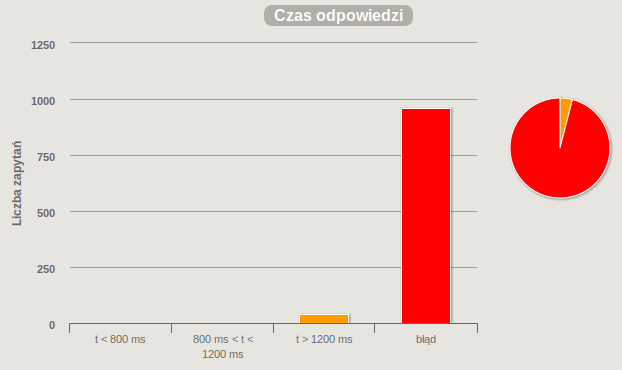
\includegraphics[resolution=150]{test_results/js/fibonacci/screenshots/response_times.png}
\caption{Wykres czasu odpowiedzi na zapytania (źródło: praca własna)}
\end{figure}

96\% zapytań zostało oznaczonych jako błędne ze względu na przekroczenie
czasu żądania wynoszącego 60 sekund. Wykorzystana biblioteka
\emph{bignum} jest implementacją natywną. Ze względu na charakterystykę
zadania, wykonywanie jest wiele operacji na dużych liczbach. Z tego
powodu silnik V8 języka JavaScript jest zmuszony do wykonywania ciągłych
odwołań do natywnego kodu, co znaczenie spowalnia pracę aplikacji.

\begin{figure}[htbp]
\centering
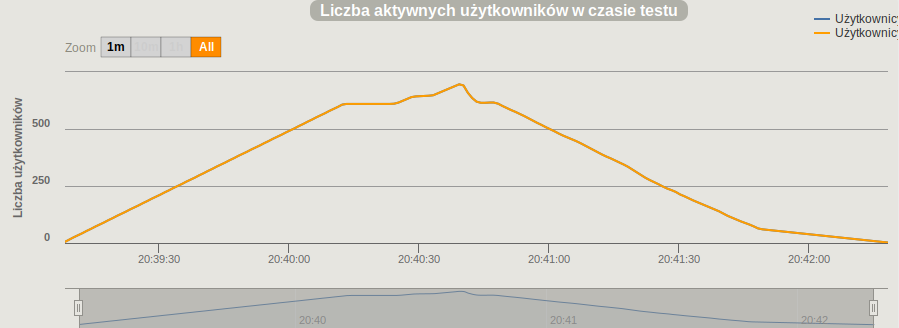
\includegraphics[resolution=150]{test_results/js/fibonacci/screenshots/active_users.png}
\caption{Wykres aktywnych użytkowników w czasie trwania testu (źródło: praca własna)}
\end{figure}

\begin{figure}[htbp]
\centering
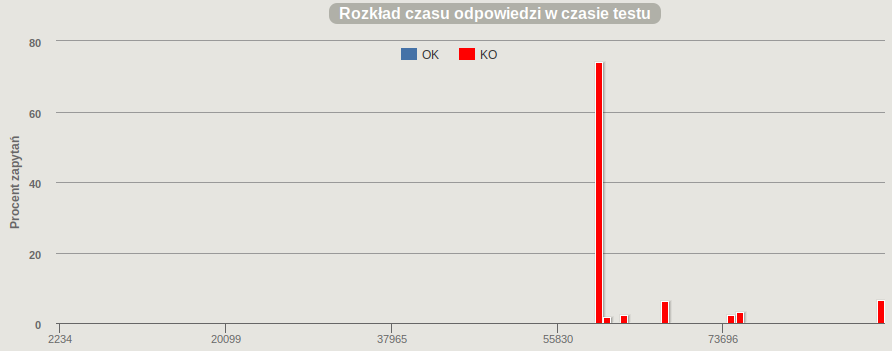
\includegraphics[resolution=150]{test_results/js/fibonacci/screenshots/distribution.png}
\caption{Wykres rozkładu czasu odpowiedzi w czasie testu (źródło: praca własna)}
\end{figure}

\begin{figure}[htbp]
\centering
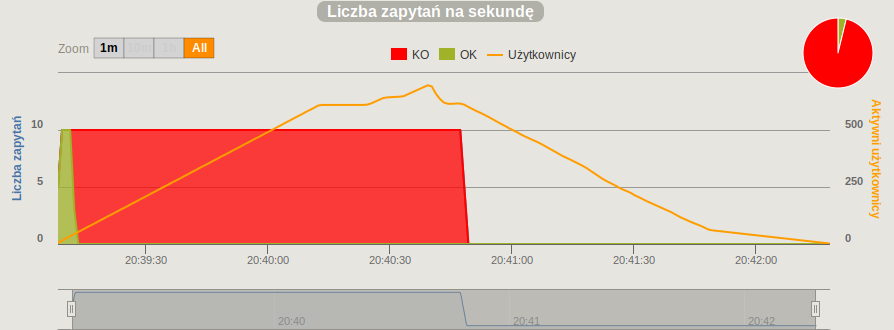
\includegraphics[resolution=150]{test_results/js/fibonacci/screenshots/requests.png}
\caption{Wykres liczby zapytań na sekundę w czasie testu (źródło: praca własna)}
\end{figure}

\begin{figure}[htbp]
\centering
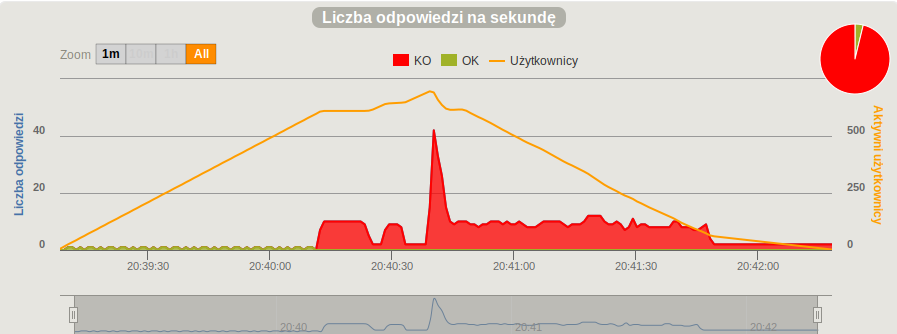
\includegraphics[resolution=150]{test_results/js/fibonacci/screenshots/responses.png}
\caption{Wykres liczby odpowiedzi na sekundę w czasie trwania testu (źródło: praca własna)}
\end{figure}

\begin{figure}[htbp]
\centering
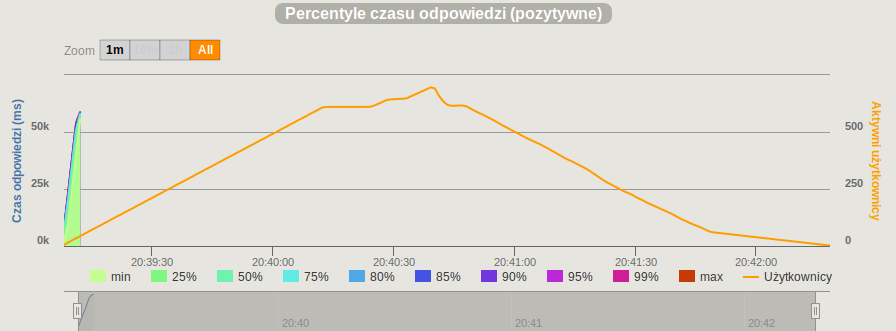
\includegraphics[resolution=150]{test_results/js/fibonacci/screenshots/response_percentile.png}
\caption{Wykres percentyli czasu odpowiedzi w czasie trwania testu (źródło: praca własna)}
\end{figure}

\begin{figure}[htbp]
\centering
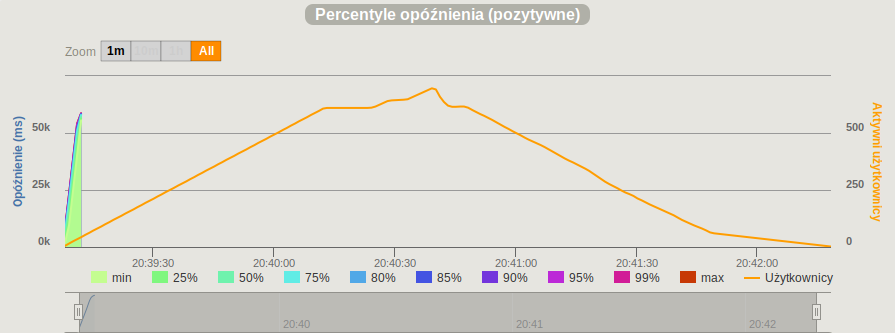
\includegraphics[resolution=150]{test_results/js/fibonacci/screenshots/latency_percentile.png}
\caption{Wykres percentyli opóźnienia w czasie trwania testu (źródło: praca własna)}
\end{figure}

\begin{longtable}[c]{@{}llll@{}}
\caption{Statystyki JavaScript w teście z wykorzystaniem czasochłonnych
obliczeń}\tabularnewline
\toprule
& W sumie & OK & KO\tabularnewline
\midrule
\endfirsthead
\toprule
& W sumie & OK & KO\tabularnewline
\midrule
\endhead
Zapytania & 1000 & 38 & 962\tabularnewline
Średnia l./s & 5,249 & 0,199 & 5,05\tabularnewline
& & &\tabularnewline
Min & 1787 & 1787 & 60000\tabularnewline
50 percentyl & 60005 & 30198 & 60004\tabularnewline
75 percentyl & 60006 & 44441 & 60006\tabularnewline
95 percentyl & 91075 & 55782 & 91075\tabularnewline
99 percentyl & 91104 & 58082 & 91104\tabularnewline
Max & 91115 & 58662 & 91115\tabularnewline
Średnia & 62260 & 30188 & 63527\tabularnewline
Odchylenie standardowe & 10900 & 16884 & 8367\tabularnewline
\bottomrule
\end{longtable}

\clearpage

\subsubsection{Elixir}\label{elixir-1}

\begin{lstlisting}[numbers=left, caption=Elixir - obliczanie n-tego elementu ciągu Fibonacciego]
defmodule Test.Calculation.Fibonacci do
    def calculate_nth(0), do: 0
    def calculate_nth(1), do: 1
    def calculate_nth(n), do: fib(0, 1, n-2)
 
    defp fib(_, prv, -1), do: prv
    defp fib(prvprv, prv, n) do
        next = prv + prvprv
        fib(prv, next, n-1)
    end
end
\end{lstlisting}

W języku Elixir, z racji jego funkcyjnego charakteru, nie istnieje
pojęcie pętli. Z tego względu wykorzystano rekurencyjną wersję
algorytmu. Użyto \emph{rekurencji ogonowej} (\emph{rekurencji
prawostronnej}, ang. \emph{tail call}), która umożliwia automatyczną
optymalizację kodu rekurencyjnego do wersji iteracyjnej. Zabieg ten
zwiększa wydajność i eliminuje zagrożenie przepełnienia stosu.

\begin{figure}[htbp]
\centering
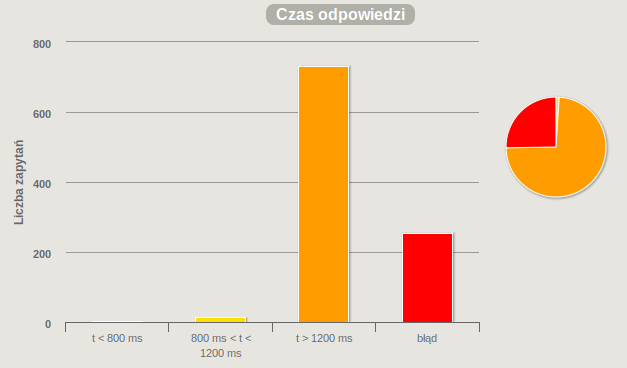
\includegraphics[resolution=150]{test_results/elixir/fibonacci/screenshots/response_times.png}
\caption{Wykres czasu odpowiedzi na zapytania (źródło: praca własna)}
\end{figure}

1/3 zapytań została oznaczona jako błędne ze względu na przekroczenie
maksymalnego czasu żądania wynoszącego 60 sekund. Poprawne odpowiedzi
otrzymano w czasie powyżej 1200 milisekund. Jedynie nieznaczną część z
nich otrzymano poniżej 1200 milisekund.

\begin{figure}[htbp]
\centering
\includegraphics[resolution=150]{test_results/elixir/fibonacci/screenshots/active_users.png}
\caption{Wykres aktywnych użytkowników w czasie trwania testu (źródło: praca własna)}
\end{figure}

\begin{figure}[htbp]
\centering
\includegraphics[resolution=150]{test_results/elixir/fibonacci/screenshots/distribution.png}
\caption{Wykres rozkładu czasu odpowiedzi w czasie testu (źródło: praca własna)}
\end{figure}

\begin{figure}[htbp]
\centering
\includegraphics[resolution=150]{test_results/elixir/fibonacci/screenshots/requests.png}
\caption{Wykres liczby zapytań na sekundę w czasie testu (źródło: praca własna)}
\end{figure}

W połowie testu obciążony system ograniczył przyjmowanie nadchodzących
zapytań czego rezultatem są zwrócone błędy.

\begin{figure}[htbp]
\centering
\includegraphics[resolution=150]{test_results/elixir/fibonacci/screenshots/responses.png}
\caption{Wykres liczby odpowiedzi na sekundę w czasie trwania testu (źródło: praca własna)}
\end{figure}

\begin{figure}[htbp]
\centering
\includegraphics[resolution=150]{test_results/elixir/fibonacci/screenshots/response_percentile.png}
\caption{Wykres percentyli czasu odpowiedzi w czasie trwania testu (źródło: praca własna)}
\end{figure}

\begin{figure}[htbp]
\centering
\includegraphics[resolution=150]{test_results/elixir/fibonacci/screenshots/latency_percentile.png}
\caption{Wykres percentyli opóźnienia w czasie trwania testu (źródło: praca własna)}
\end{figure}

\begin{longtable}[c]{@{}llll@{}}
\caption{Statystyki Elixir w teście z wykorzystaniem czasochłonnych
obliczeń}\tabularnewline
\toprule
& W sumie & OK & KO\tabularnewline
\midrule
\endfirsthead
\toprule
& W sumie & OK & KO\tabularnewline
\midrule
\endhead
Zapytania & 1 000,00 & 747,00 & 253,00\tabularnewline
Średnia l./s & 6,26 & 4,68 & 1,585\tabularnewline
& & &\tabularnewline
Min & 484 & 484 & 60008\tabularnewline
50 percentyl & 46684 & 35390 & 60009\tabularnewline
75 percentyl & 60008 & 48516 & 60009\tabularnewline
95 percentyl & 60008 & 56588 & 60009\tabularnewline
99 percentyl & 60009 & 59529 & 60010\tabularnewline
Max & 60010 & 59975 & 60010\tabularnewline
Średnia & 40075 & 33324 & 60008\tabularnewline
Odchylenie standardowe & 18823 & 17152 & 0\tabularnewline
\bottomrule
\end{longtable}

\clearpage

\subsection{Operacje na zbiorach
danych}\label{operacje-na-zbiorach-danych}

Zadaniem testu \ref{czasochux142onne-obliczenia} było zbadanie
zachowania systemu przy dużej liczby wykonywanych operacji na każde
otrzymane żądanie. Celem tego testu jest porównanie każdej z wybranych
technologii w kategorii możliwości manipulowania danymi pod obciążeniem.

Test polega na wykonaniu metody HTTP POST, w ciele której umieszczono
wygenerowaną macierz liczb całkowitych o rozmiarze 100 na 100. Zadaniem
serwera jest zwrócenie w odpowiedzi transponowanej macierzy.
Zasymulowano 10000 użytkowników wykonujących zapytanie niezależnie,
rozłożonych na przestrzeni 100 sekund.

\subsubsection{Java}\label{java-2}

\begin{lstlisting}[language=Java, numbers=left, caption=Java - transpozycja macierzy]
public class Matrix {
    public static int[][] transpose(int [][] matrix) {
        int xDimension = matrix.length;
        int yDimension = matrix[0].length;

        int[][] result = new int[yDimension][xDimension];
        for (int row = 0; row < xDimension; row++) {
            for (int col = 0; col < yDimension; col++) {
                result[col][row] = matrix[row][col];
            }
        }

        return result;
    }
}
\end{lstlisting}

Powyższy kod pobiera wymiary \(x, y\) przekazanej macierzy \(a\), aby
utworzyć nową macierz \(b\) o wymiarach \(y, x\). Następnie, wiersz po
wierszu i element po elemencie z każdego wiersza, wartości macierzy
\(a\) są przepisywane do macierzy \(b\), tak aby \(a_{xy} = b_{yx}\)

\begin{figure}[htbp]
\centering
\includegraphics[resolution=150]{test_results/java/matrix/screenshots/response_times.png}
\caption{Wykres czasu odpowiedzi na zapytania (źródło: praca własna)}
\end{figure}

Korzystając z implementacji w języku Java żadne z zapytań nie zwróciło
błędu. Na 99\% żądań odpowiedź otrzymano poniżej 800 milisekund, a
jedynie 83 z nich przetworzono powyżej tej granicy.

\begin{figure}[htbp]
\centering
\includegraphics[resolution=150]{test_results/java/matrix/screenshots/active_users.png}
\caption{Wykres aktywnych użytkowników w czasie trwania testu (źródło: praca własna)}
\end{figure}

\begin{figure}[htbp]
\centering
\includegraphics[resolution=150]{test_results/java/matrix/screenshots/distribution.png}
\caption{Wykres rozkładu czasu odpowiedzi w czasie testu (źródło: praca własna)}
\end{figure}

\begin{figure}[htbp]
\centering
\includegraphics[resolution=150]{test_results/java/matrix/screenshots/requests.png}
\caption{Wykres liczby zapytań na sekundę w czasie testu (źródło: praca własna)}
\end{figure}

\begin{figure}[htbp]
\centering
\includegraphics[resolution=150]{test_results/java/matrix/screenshots/responses.png}
\caption{Wykres liczby odpowiedzi na sekundę w czasie trwania testu (źródło: praca własna)}
\end{figure}

Zauważono ubytek, a zaraz po nim skok liczby odpowiedzi na sekundę w
początkowej fazie testu. Po wstępnej inicjalizacji aplikacji, każdy nowy
użytkownik został obsłużony na bieżąco.

\begin{figure}[htbp]
\centering
\includegraphics[resolution=150]{test_results/java/matrix/screenshots/response_percentile.png}
\caption{Wykres percentyli czasu odpowiedzi w czasie trwania testu (źródło: praca własna)}
\end{figure}

\begin{figure}[htbp]
\centering
\includegraphics[resolution=150]{test_results/java/matrix/screenshots/latency_percentile.png}
\caption{Wykres percentyli opóźnienia w czasie trwania testu (źródło: praca własna)}
\end{figure}

Wystąpiła niewielka różnica w czasach odpowiedzi i opóźnienia pomiędzy
poszczególnymi zapytaniami w czasie trwania testu.

\begin{longtable}[c]{@{}llll@{}}
\caption{Statystyki Java w teście z wykorzystaniem zbiorów
danych}\tabularnewline
\toprule
& W sumie & OK & KO\tabularnewline
\midrule
\endfirsthead
\toprule
& W sumie & OK & KO\tabularnewline
\midrule
\endhead
Zapytania & 10000 & 10000 & 0\tabularnewline
Średnia l./s & 99,785 & 99,785 & -\tabularnewline
& & &\tabularnewline
Min & 5 & 5 & -\tabularnewline
50 percentyl & 209 & 209 & -\tabularnewline
75 percentyl & 210 & 210 & -\tabularnewline
95 percentyl & 214 & 214 & -\tabularnewline
99 percentyl & 815 & 815 & -\tabularnewline
Max & 1418 & 1418 & -\tabularnewline
Średnia & 162 & 162 & -\tabularnewline
Odchylenie standardowe & 137 & 137 & -\tabularnewline
\bottomrule
\end{longtable}

\clearpage

\subsubsection{JavaScript}\label{javascript-2}

\begin{lstlisting}[numbers=left, caption=JavaScript - transpozycja macierzy]
function transpose(matrix) {
    var xDimension = matrix.length;
    var yDimension = matrix[0].length;

    var result = [];
    for (var row = 0; row < xDimension; row++) {
        var new_row = [];
        for (var col = 0; col < yDimension; col++) {
            new_row.push(matrix[col][row]);
        }
        result.push(new_row);
    }

    return result;
}
\end{lstlisting}

Implementacja ta jest translacją z języka Java, jednak każdy z wierszy
jest tworzony i uzupełniany niezależnie, a następnie dołączany na koniec
macierzy wynikowej.

\begin{figure}[htbp]
\centering
\includegraphics[resolution=150]{test_results/js/matrix/screenshots/response_times.png}
\caption{Wykres czasu odpowiedzi na zapytania (źródło: praca własna)}
\end{figure}

78\% ze wszystkich zapytań zostało obsłużonych poniżej 800 milisekund
oraz żadne nie przekroczyło granicy 1200 milisekund czasu odpowiedzi.

\begin{figure}[htbp]
\centering
\includegraphics[resolution=150]{test_results/js/matrix/screenshots/active_users.png}
\caption{Wykres aktywnych użytkowników w czasie trwania testu (źródło: praca własna)}
\end{figure}

\begin{figure}[htbp]
\centering
\includegraphics[resolution=150]{test_results/js/matrix/screenshots/distribution.png}
\caption{Wykres rozkładu czasu odpowiedzi w czasie testu (źródło: praca własna)}
\end{figure}

\begin{figure}[htbp]
\centering
\includegraphics[resolution=150]{test_results/js/matrix/screenshots/requests.png}
\caption{Wykres liczby zapytań na sekundę w czasie testu (źródło: praca własna)}
\end{figure}

\begin{figure}[htbp]
\centering
\includegraphics[resolution=150]{test_results/js/matrix/screenshots/responses.png}
\caption{Wykres liczby odpowiedzi na sekundę w czasie trwania testu (źródło: praca własna)}
\end{figure}

Wszystkie żądania przyjęto niezwłocznie do obsługi, zaś wykres czasu
odpowiedzi przedstawia niemalże cykliczne skoki. Node.js operuje jednym
wątkiem w jednym procesie. W czasie testu system operacyjny starał się
zbalansować pracę obydwu dostępnych rdzeni procesora przenosząc
obciążenie pomiędzy nimi.

\begin{figure}[htbp]
\centering
\includegraphics[resolution=150]{test_results/js/matrix/screenshots/response_percentile.png}
\caption{Wykres percentyli czasu odpowiedzi w czasie trwania testu (źródło: praca własna)}
\label{js:matrix:response_percentile}
\end{figure}

\begin{figure}[htbp]
\centering
\includegraphics[resolution=150]{test_results/js/matrix/screenshots/latency_percentile.png}
\caption{Wykres percentyli opóźnienia w czasie trwania testu (źródło: praca własna)}
\label{js:matrix:latency_percentile}
\end{figure}

Na podstawie wykresów \ref{js:matrix:response_percentile} oraz
\ref{js:matrix:latency_percentile} można zaobserwować wpływ
optymalizacji przetwarzania zapytań przez silnik V8. Czas odpowiedzi,
jak i opóźnienie wyraźnie spada podczas trwania testu.

\begin{longtable}[c]{@{}llll@{}}
\caption{Statystyki JavaScript w teście z wykorzystaniem zbiorów
danych}\tabularnewline
\toprule
& W sumie & OK & KO\tabularnewline
\midrule
\endfirsthead
\toprule
& W sumie & OK & KO\tabularnewline
\midrule
\endhead
Zapytania & 10000 & 10000 & 0\tabularnewline
Średnia l./s & 99,743 & 99,743 & -\tabularnewline
& & &\tabularnewline
Min & 219 & 219 & -\tabularnewline
50 percentyl & 655 & 655 & -\tabularnewline
75 percentyl & 779 & 779 & -\tabularnewline
95 percentyl & 1002 & 1001 & -\tabularnewline
99 percentyl & 1102 & 1102 & -\tabularnewline
Max & 1161 & 1161 & -\tabularnewline
Średnia & 644 & 644 & -\tabularnewline
Odchylenie standardowe & 203 & 203 & -\tabularnewline
\bottomrule
\end{longtable}

\clearpage

\subsubsection{Elixir}\label{elixir-2}

\begin{lstlisting}[numbers=left, caption=Elixir - transpozycja macierzy]
defmodule Test.Calculation.Matrix do
    def transpose(matrix) do
        matrix |>
        List.zip |>
        Enum.map(&Tuple.to_list(&1))
    end
end
\end{lstlisting}

Transpozycja macierzy w języku Elixir korzysta z jego funkcyjnych
możliwości. Dzięki użyciu funkcji dostępnych w standardowej bibliotece
kod jest bardziej zwięzły od pozostałych implementacji. Funkcja
\emph{List.zip} łączy w krotki elementy z każdego wiersza macierzy o tej
samej pozycji. Następnie, używając funkcji \emph{Enum.map}, na każdej z
utworzonych krotek wykonywana jest funkcja \emph{Tuple.to\_list}, w celu
przekształcenia ich do jednorodnej macierzy.

\begin{figure}[htbp]
\centering
\includegraphics[resolution=150]{test_results/elixir/matrix/screenshots/response_times.png}
\caption{Wykres czasu odpowiedzi na zapytania (źródło: praca własna)}
\end{figure}

Błędne zapytania stanowią 7\% całego testu, pozostałe zaś zostały
przetworzone w czasie powyżej 1200 milisekund.

\begin{figure}[htbp]
\centering
\includegraphics[resolution=150]{test_results/elixir/matrix/screenshots/active_users.png}
\caption{Wykres aktywnych użytkowników w czasie trwania testu (źródło: praca własna)}
\end{figure}

\begin{figure}[htbp]
\centering
\includegraphics[resolution=150]{test_results/elixir/matrix/screenshots/distribution.png}
\caption{Wykres rozkładu czasu odpowiedzi w czasie testu (źródło: praca własna)}
\end{figure}

\begin{figure}[htbp]
\centering
\includegraphics[resolution=150]{test_results/elixir/matrix/screenshots/requests.png}
\caption{Wykres liczby zapytań na sekundę w czasie testu (źródło: praca własna)}
\end{figure}

Liczba przyjmowanych żądań na sekundę utrzymywała się na stałym
poziomie. Jednak, część zapytań, ze względu na obciążenie została
odrzucona, a odpowiedzi na nie przekroczyły maksymalny czas żądania
wynoszący 60 sekund.

\begin{figure}[htbp]
\centering
\includegraphics[resolution=150]{test_results/elixir/matrix/screenshots/responses.png}
\caption{Wykres liczby odpowiedzi na sekundę w czasie trwania testu (źródło: praca własna)}
\end{figure}

\begin{figure}[htbp]
\centering
\includegraphics[resolution=150]{test_results/elixir/matrix/screenshots/response_percentile.png}
\caption{Wykres percentyli czasu odpowiedzi w czasie trwania testu (źródło: praca własna)}
\end{figure}

\begin{figure}[htbp]
\centering
\includegraphics[resolution=150]{test_results/elixir/matrix/screenshots/latency_percentile.png}
\caption{Wykres percentyli opóźnienia w czasie trwania testu (źródło: praca własna)}
\end{figure}

Pomimo utraty części zapytań w granicach 19:37:25 czas odpowiedzi oraz
opóźnienie uległy poprawie.

\begin{longtable}[c]{@{}llll@{}}
\caption{Statystyki Elixir w teście z wykorzystaniem zbiorów
danych}\tabularnewline
\toprule
& W sumie & OK & KO\tabularnewline
\midrule
\endfirsthead
\toprule
& W sumie & OK & KO\tabularnewline
\midrule
\endhead
Zapytania & 10000 & 9274 & 726\tabularnewline
Średnia l./s & 65,691 & 60,922 & 4,769\tabularnewline
& & &\tabularnewline
Min & 443 & 443 & 38129\tabularnewline
50 percentyl & 17306 & 16997 & 60004\tabularnewline
75 percentyl & 23553 & 21548 & 60005\tabularnewline
95 percentyl & 60004 & 41425 & 60006\tabularnewline
99 percentyl & 60005 & 47648 & 62513\tabularnewline
Max & 75051 & 55303 & 75051\tabularnewline
Średnia & 22038 & 19058 & 60103\tabularnewline
Odchylenie standardowe & 14021 & 9461 & 1518\tabularnewline
\bottomrule
\end{longtable}

\clearpage

\subsection{Ograniczenia
wejścia/wyjścia}\label{ograniczenia-wejux15bciawyjux15bcia}

Większość systemów informatycznych korzysta z pewnego rodzaju urządzeń
wejścia/wyjścia. Nie licząc urządzenia sieciowego, używanymi
interfejsami mogą być system plików czy system zarządzania bazą danych.
W tym teście wykorzystano system plików, gdyż jest obsługiwany przez
standardową bibliotekę każdej z porównywanych technologii, w
przeciwieństwie do komunikacji z bazą danych.

Test polega na wykonaniu metody HTTP GET na serwerze zwracającym plik
tekstowy ze znakami ASCI o rozmiarze 1MB. Zasymulowano 12000
użytkowników wykonujących zapytanie niezależnie, rozłożonych na
przestrzeni 100 sekund.

Implementacje we wszystkich trzech technologiach są trywialne,
korzystają ze standardowej biblioteki do umieszczenia pliku w ciele
odpowiedzi, więc zostały pominięte.

\subsubsection{Java}\label{java-3}

\begin{figure}[htbp]
\centering
\includegraphics[resolution=150]{test_results/java/file/screenshots/response_times.png}
\caption{Wykres czasu odpowiedzi na zapytania (źródło: praca własna)}
\end{figure}

Nie utracono żadnego żądania i żadna odpowiedź nie została oznaczona
jako błędna, lecz 100\% z nich otrzymano w czasie większym niż 1200
milisekund.

\begin{figure}[htbp]
\centering
\includegraphics[resolution=150]{test_results/java/file/screenshots/active_users.png}
\caption{Wykres aktywnych użytkowników w czasie trwania testu (źródło: praca własna)}
\end{figure}

Liczba aktywnych użytkowników rośnie jednostajnie ze względu na
oczekiwanie na obsługę poprzedzających zapytań.

\begin{figure}[htbp]
\centering
\includegraphics[resolution=150]{test_results/java/file/screenshots/distribution.png}
\caption{Wykres rozkładu czasu odpowiedzi w czasie testu (źródło: praca własna)}
\end{figure}

\begin{figure}[htbp]
\centering
\includegraphics[resolution=150]{test_results/java/file/screenshots/requests.png}
\caption{Wykres liczby zapytań na sekundę w czasie testu (źródło: praca własna)}
\end{figure}

\begin{figure}[htbp]
\centering
\includegraphics[resolution=150]{test_results/java/file/screenshots/responses.png}
\caption{Wykres liczby odpowiedzi na sekundę w czasie trwania testu (źródło: praca własna)}
\end{figure}

Serwer utrzymał stały poziom obsługi przychodzących połączeń oraz
odpowiedzi.

\begin{figure}[htbp]
\centering
\includegraphics[resolution=150]{test_results/java/file/screenshots/response_percentile.png}
\caption{Wykres percentyli czasu odpowiedzi w czasie trwania testu (źródło: praca własna)}
\end{figure}

\begin{figure}[htbp]
\centering
\includegraphics[resolution=150]{test_results/java/file/screenshots/latency_percentile.png}
\caption{Wykres percentyli opóźnienia w czasie trwania testu (źródło: praca własna)}
\end{figure}

Czas odpowiedzi oraz opóźnienie pokrywają się z liczbą aktywnych
użytkowników. Wraz ze wzrostem liczby oczekujących zapytań wzrasta czas
odpowiedzi oraz opóźnienie. Wystąpiło nieznaczne rozwarstwienie w
czasach odpowiedzi w danej chwili czasu testu.

\begin{longtable}[c]{@{}llll@{}}
\caption{Statystyki Java w teście z ograniczeniami
wejścia/wyjścia}\tabularnewline
\toprule
& W sumie & OK & KO\tabularnewline
\midrule
\endfirsthead
\toprule
& W sumie & OK & KO\tabularnewline
\midrule
\endhead
Zapytania & 12000 & 12000 & 0\tabularnewline
Średnia l./s & 115,657 & 115,657 & -\tabularnewline
& & &\tabularnewline
Min & 1067 & 1067 & -\tabularnewline
50 percentyl & 2611 & 2611 & -\tabularnewline
75 percentyl & 3252 & 3252 & -\tabularnewline
95 percentyl & 3782 & 3782 & -\tabularnewline
99 percentyl & 3882 & 3882 & -\tabularnewline
Max & 4233 & 4233 & -\tabularnewline
Średnia & 2606 & 2606 & -\tabularnewline
Odchylenie standardowe & 759 & 759 & -\tabularnewline
\bottomrule
\end{longtable}

\clearpage

\subsubsection{JavaScript}\label{javascript-3}

\begin{figure}[htbp]
\centering
\includegraphics[resolution=150]{test_results/js/file/screenshots/response_times.png}
\caption{Wykres czasu odpowiedzi na zapytania (źródło: praca własna)}
\end{figure}

Na 10\% z otrzymanych zapytań serwer odpowiedział w czasie poniżej 800
milisekund, na kolejnych 9\% w czasie pomiędzy 800 a 1200 milisekund,
zaś pozostałe powyżej 1200 milisekund.

\begin{figure}[htbp]
\centering
\includegraphics[resolution=150]{test_results/js/file/screenshots/active_users.png}
\caption{Wykres aktywnych użytkowników w czasie trwania testu (źródło: praca własna)}
\end{figure}

Liczba aktywnych użytkowników rośnie jednostajnie ze względu na
oczekiwanie na obsługę poprzedzających zapytań.

\begin{figure}[htbp]
\centering
\includegraphics[resolution=150]{test_results/js/file/screenshots/distribution.png}
\caption{Wykres rozkładu czasu odpowiedzi w czasie testu (źródło: praca własna)}
\end{figure}

\begin{figure}[htbp]
\centering
\includegraphics[resolution=150]{test_results/js/file/screenshots/requests.png}
\caption{Wykres liczby zapytań na sekundę w czasie testu (źródło: praca własna)}
\end{figure}

\begin{figure}[htbp]
\centering
\includegraphics[resolution=150]{test_results/js/file/screenshots/responses.png}
\caption{Wykres liczby odpowiedzi na sekundę w czasie trwania testu (źródło: praca własna)}
\end{figure}

Zarówno liczbę zapytań jak i odpowiedzi utrzymano na stałym poziomie.

\begin{figure}[htbp]
\centering
\includegraphics[resolution=150]{test_results/js/file/screenshots/response_percentile.png}
\caption{Wykres percentyli czasu odpowiedzi w czasie trwania testu (źródło: praca własna)}
\end{figure}

\begin{figure}[htbp]
\centering
\includegraphics[resolution=150]{test_results/js/file/screenshots/latency_percentile.png}
\caption{Wykres percentyli opóźnienia w czasie trwania testu (źródło: praca własna)}
\end{figure}

Czas odpowiedzi oraz opóźnienie rosną wraz z wzrastającą liczbą
aktywnych użytkowników, oczekujących na odpowiedź. Opóźnienia oraz czasy
odpowiedzi w danej chwili czasu są niejednorodne, rozwarstwienie rośnie
w miarę przybywania aktywnych użytkowników.

\begin{longtable}[c]{@{}llll@{}}
\caption{Statystyki JavaScript w teście z ograniczeniami
wejścia/wyjścia}\tabularnewline
\toprule
& W sumie & OK & KO\tabularnewline
\midrule
\endfirsthead
\toprule
& W sumie & OK & KO\tabularnewline
\midrule
\endhead
Zapytania & 12000 & 12000 & 0\tabularnewline
Średnia l./s & 114,718 & 114,718 & -\tabularnewline
& & &\tabularnewline
Min & 248 & 248 & -\tabularnewline
50 percentyl & 2461 & 2461 & -\tabularnewline
75 percentyl & 3632 & 3631 & -\tabularnewline
95 percentyl & 7101 & 7101 & -\tabularnewline
99 percentyl & 10849 & 10849 & -\tabularnewline
Max & 22763 & 22763 & -\tabularnewline
Średnia & 2921 & 2921 & -\tabularnewline
Odchylenie standardowe & 2162 & 2162 & -\tabularnewline
\bottomrule
\end{longtable}

\clearpage

\subsubsection{Elixir}\label{elixir-3}

\begin{figure}[htbp]
\centering
\includegraphics[resolution=150]{test_results/elixir/file/screenshots/response_times.png}
\caption{Wykres czasu odpowiedzi na zapytania (źródło: praca własna)}
\end{figure}

Zaledwie 2\% zapytań obsłużono w czasie poniżej 800 milisekund, 90\%
całości powyżej 1200 milisekund, pozostałe żądania trafiły pomiędzy te
dwie grupy. Żadna z odpowiedzi nie została oznaczona błędem.

\begin{figure}[htbp]
\centering
\includegraphics[resolution=150]{test_results/elixir/file/screenshots/active_users.png}
\caption{Wykres aktywnych użytkowników w czasie trwania testu (źródło: praca własna)}
\end{figure}

Liczba aktywnych użytkowników rośnie jednostajnie ze względu na
oczekiwanie na obsługę poprzedzających zapytań.

\begin{figure}[htbp]
\centering
\includegraphics[resolution=150]{test_results/elixir/file/screenshots/distribution.png}
\caption{Wykres rozkładu czasu odpowiedzi w czasie testu (źródło: praca własna)}
\end{figure}

\begin{figure}[htbp]
\centering
\includegraphics[resolution=150]{test_results/elixir/file/screenshots/requests.png}
\caption{Wykres liczby zapytań na sekundę w czasie testu (źródło: praca własna)}
\end{figure}

\begin{figure}[htbp]
\centering
\includegraphics[resolution=150]{test_results/elixir/file/screenshots/responses.png}
\caption{Wykres liczby odpowiedzi na sekundę w czasie trwania testu (źródło: praca własna)}
\end{figure}

Utrzymano stały poziom poziom obsługi połączeń przychodzących oraz
przetwarzania odpowiedzi.

\begin{figure}[htbp]
\centering
\includegraphics[resolution=150]{test_results/elixir/file/screenshots/response_percentile.png}
\caption{Wykres percentyli czasu odpowiedzi w czasie trwania testu (źródło: praca własna)}
\end{figure}

\begin{figure}[htbp]
\centering
\includegraphics[resolution=150]{test_results/elixir/file/screenshots/latency_percentile.png}
\caption{Wykres percentyli opóźnienia w czasie trwania testu (źródło: praca własna)}
\end{figure}

Czas odpowiedzi oraz opóźnienie rosną wraz z wzrastającą liczbą
aktywnych użytkowników, oczekujących na odpowiedź. Opóźnienia oraz czasy
odpowiedzi w danej chwili czasu są niejednorodne, rozwarstwienie rośnie
w miarę przybywania aktywnych użytkowników.

\begin{longtable}[c]{@{}llll@{}}
\caption{Statystyki Elixir w teście z ograniczeniami
wejścia/wyjścia}\tabularnewline
\toprule
& W sumie & OK & KO\tabularnewline
\midrule
\endfirsthead
\toprule
& W sumie & OK & KO\tabularnewline
\midrule
\endhead
Zapytania & 12000 & 12000 & 0\tabularnewline
Średnia l./s & 116,457 & 116,457 & -\tabularnewline
& & &\tabularnewline
Min & 639 & 639 & -\tabularnewline
50 percentyl & 2797 & 2797 & -\tabularnewline
75 percentyl & 3988 & 3988 & -\tabularnewline
95 percentyl & 7900 & 7900 & -\tabularnewline
99 percentyl & 11616 & 11616 & -\tabularnewline
Max & 21174 & 21174 & -\tabularnewline
Średnia & 3342 & 3342 & -\tabularnewline
Odchylenie standardowe & 2239 & 2239 & -\tabularnewline
\bottomrule
\end{longtable}

\clearpage

\subsection{Podsumowanie}\label{podsumowanie}

\begin{figure}[!ht]
\centering
\includegraphics[resolution=120]{test_results/summary/simple_avg.png}
\caption{Wykres średniej liczby zapytań dla prostych zapytań}
\end{figure}

W przypadku testu dużej liczby jednoczesnych zapytań najlepszy wynik
otrzymał Elixir. Osiągnął 3498,74 żądań na sekundę, a żadne z nich nie
otrzymało błędnej odpowiedzi. Zastosowanie modelu aktorowego do obsługi
zapytań sprowadza się do oddelegowania każdego przychodzącego żądania do
nowego aktora. Strategia ta wypadła lepiej od odpowiednika w Javie,
zakładającego wykorzystywanie wątków systemu operacyjnego do
przetwarzania zapytań. Najgorszy wynik otrzymano przy użyciu JavaScript.
Średnia liczba otrzymanych błędnych odpowiedzi niewiele różni się
pomiędzy Javą i JavaScriptem, lecz przy 74\% wydajności JavaScriptu
względem Javy.

\begin{figure}[!ht]
\centering
\includegraphics[resolution=120]{test_results/summary/simple_percentage.png}
\caption{Wykres poprawnej wymiany zapytań i odpowiedzi dla prostych zapytań}
\end{figure}

\begin{figure}[!ht]
\centering
\includegraphics[resolution=120]{test_results/summary/simple_response.png}
\caption{Wykres czasu odpowiedzi dla prostych zapytań}
\end{figure}

W tym przypadku znaczący wpływ wywarła optymalizacja w czasie
wykonywania programu. Czasy odpowiedzi pierwszych 20 sekund
przetwarzania w Elixirze, chociaż niższe od ekwiwalentnych w Javie i
JavaScripcie, są nieporównywalnie wyższe od kolejnych. Wirtualna maszyna
Erlanga wykryła powtarzający się wzorzec i stworzyła optymalny kod dla
tego przypadku. Powtórne testy wykazały takie same wyniki w każdej z
prób. Średni czas odpowiedzi dla Javy i JavaScriptu jest porównywalny, z
nieznaczącą przewagą pierwszej technologii. Rezultat ten odbił się na
odchyleniu standardowym ze względu na wyższy czas maksymalny w Javie.

\begin{figure}[!ht]
\centering
\includegraphics[resolution=120]{test_results/summary/fib_avg.png}
\caption{Wykres średniej liczby zapytań dla wyliczenia liczby ciągu Fibonacciego}
\end{figure}

W grupie czasochłonnych obliczeń, dla przypadku obliczania liczby
Fibonacciego, pomimo zbliżonej średniej liczbie zapytań na sekundę
pomiędzy Javą i Elixirem, Elixir osiągnął lepszy wynik pod względem
średniej liczby zapytań na sekundę oraz odsetka błędnych odpowiedzi.
Procent poprawnie przetworzonych zapytań Javy i JavaScriptu, odpowiednio
26\% i 4\%, jest nieporównywalny z 75\% Elixira.

\begin{figure}[!ht]
\centering
\includegraphics[resolution=120]{test_results/summary/fib_percentage.png}
\caption{Wykres poprawnej wymiany zapytań i odpowiedzi dla wyliczenia liczby ciągu Fibonacciego}
\end{figure}

\begin{figure}[!ht]
\centering
\includegraphics[resolution=120]{test_results/summary/fib_response.png}
\caption{Wykres czasu odpowiedzi dla wyliczenia liczby ciągu Fibonacciego}
\label{summary:fib:response}
\end{figure}

Czasy odpowiedzi dla każdej z trzech testowanych technologii plasują się
na podobnym poziomie, z różnicami jedynie w czasach minimalnych. Należy
jednak wziąć pod uwagę fakt, że rysunek \ref{summary:fib:response}
przedstawia wyniki jedynie dla odpowiedzi poprawnych. W przypadku
technologii Java i JavaScript wyniki mogą stanowić źródło nieprawdy,
gdyż niewielka cześć całości żądań testu została przez nie przetworzona
poprawnie.

\begin{figure}[!ht]
\centering
\includegraphics[resolution=120]{test_results/summary/matrix_avg.png}
\caption{Wykres średniej liczby zapytań dla transpozycji macierzy}
\end{figure}

W przypadku transpozycji macierzy Java oraz JavaScript uzyskały niemalże
identyczne wyniki. Rozwiązania z wykorzystaniem obu technologii
obsłużyły poprawnie wszystkie zapytania z wynikiem około 100 zapytań na
sekundę.

\begin{figure}[!ht]
\centering
\includegraphics[resolution=120]{test_results/summary/matrix_percentage.png}
\caption{Wykres poprawnej wymiany zapytań i odpowiedzi dla transpozycji macierzy}
\end{figure}

\begin{figure}[!ht]
\centering
\includegraphics[resolution=120]{test_results/summary/matrix_response.png}
\caption{Wykres czasu odpowiedzi dla transpozycji macierzy}
\end{figure}

W kategorii czasu odpowiedzi Java wypadła lepiej od JavaScript ze
średnim czasem 162 milisekund przeciwko 644 milisekundom. W tym teście
wyniki Elixira są znaczenie gorsze od dwóch pozostałych technologii
osiągając średni czas odpowiedzi równy 22038 milisekund oraz tracąc 7\%
zapytań. Tak pokaźne pogorszenie w stosunku do poprzednich testów wynika
z przyjętego modelu obliczeń. Model aktorowy, który uprzednio stanowił
atut, jest przyczyną dłuższych czasów odpowiedzi. Ze względu na fakt, że
lekkie procesy w wirtualnej maszynie Erlanga nie współdzielą stanu,
wszystkie dane pomiędzy nimi są kopiowane powodując opóźnienia. Proces
transpozycji macierzy w dużej mierze polega na przekształceniach
struktur danych. W języku Elixir wszystkie struktury danych są
niezmienne, więc w każdym kroku wykonywane są kolejne kopie danych, co
ma negatywny wpływ na wyniki.

\begin{figure}[!ht]
\centering
\includegraphics[resolution=120]{test_results/summary/file_avg.png}
\caption{Wykres średniej liczby zapytań dla odczytu pliku}
\end{figure}

W przypadku odczytu pliku wszystkie zapytania i odpowiedzi zostały
obsłużone w 100\%.

\begin{figure}[!ht]
\centering
\includegraphics[resolution=120]{test_results/summary/file_response.png}
\caption{Wykres czasu odpowiedzi dla odczytu pliku}
\end{figure}

Java uzyskała bardzo stabilne wyniki, wydajnościowo test nie stanowił
problemu, lecz ze względu na to, że dostęp do plików w Javie jest w
znacznej części blokujący, obsługa wielu z zapytań została opóźniona
przez oczekiwanie na urządzenie wejścia/wyjścia. Najniższy czas
odpowiedzi, 248 milisekund, osiągnął JavaScript, a tuż za nim, z
wynikiem 639 milisekund Elixir.

\clearpage
\clearpage{}
	\clearpage{}\section{Skalowalność}\label{skalowalnoux15bux107}

\emph{Skalowalność}, w kontekście systemów informatycznych, jest
zdolnością systemu do efektywnego wykorzystania zwiększonej puli
zasobów. Innymi słowy zwiększając możliwości obliczeniowe sprzętu, w
ramach którego oprogramowanie jest uruchomione, wydajność powinna się
zwiększyć. Można wyróżnić dwa wymiary
skalowalności\autocite{elrewini2005advanced}:

\begin{itemize}
\tightlist
\item
  pionowa
\item
  pozioma
\end{itemize}

\subsection{Skalowalność pionowa}\label{skalowalnoux15bux107-pionowa}

Mówimy o \emph{skalowalności pionowej} jeśli zwiększamy zasoby jednego
węzła systemu komputerowego, rdzenie procesora lub pamięć do jednego
komputera.\autocite{elrewini2005advanced}

Wirtualna maszyna, z której korzysta Java, jest w stanie użyć wszystkich
dostępnych rdzeni procesora. Ich wykorzystanie zależy od zastosowania
mechanizmów współbieżności dostępnych w języku, np. wątków.
Wielowątkowość JVM jest zaimplementowana z użyciem natywnych wątków
systemów operacyjnych. Dodatkowo Java udostępnia pewne abstrakcje, np.
wykonawców (ang. \emph{executor}), mające za zadanie ułatwić
programistom prace w wielowątkowym środowisku. Wirtualna maszyna Javy
oferuje zbiór parametrów konfiguracyjnych pozwalających na strojenie jej
pracy. Dzięki nim można dostosować, między innymi, wykorzystanie pamięci
operacyjnej, aby lepiej wykorzystać dostępne zasoby.

Założeniem JavaScriptu, a raczej Node.js, jest użytkowanie
jednowątkowego modelu Reaktor. W związku z tym każdy proces aplikacji
może wykorzystać tylko jeden wątek systemu operacyjnego. Standardowa
biblioteka Node'a zawiera moduł \emph{cluster}. Umożliwia on rozwidlenie
aplikacji przy użyciu komendy \emph{fork} na zasadzie
\emph{master/slave}. Proces \emph{master} jest punktem wejściowym
programu i jest odpowiedzialny za uruchomienie procesów potomnych.
Tworzone procesy, zwane \emph{worker}, odpowiadają za logikę aplikacji.
Mogą one współdzielić nasłuchiwany port, wtedy zapytania zostaną
automatycznie zbalansowane pomiędzy wszystkie procesy potomne. Zamysłem
modułu było proste, niskopoziomowe wsparcie dla wielu procesów,
programista jest odpowiedzialny za zarządzanie nimi i obsługę błędów.

Wirtualna maszyna Erlanga, BEAM, zarządza lekkimi procesami
automatycznie, zajmuje się rozdzielaniem dostępnych zasobów pomiędzy
jednostki obliczeniowe i harmonogramuje zadania. Jedyną abstrakcją ponad
wątkami są lekkie procesy wirtualnej maszyny, modelowane na aktorów. W
wypadku, gdy potrzebna jest większa kontrola nad sprzętem, niezbędne
jest wykorzystanie natywnych wywołań. Podobnie jak wirtualna maszyna
Javy, BEAM udostępnia szereg parametrów konfiguracyjnych, jednak w
przeciwieństwie do JVM umożliwia kontrolę nad wykorzystaniem procesorów.

\subsection{Skalowalność pozioma}\label{skalowalnoux15bux107-pozioma}

Mówimy o \emph{skalowalności poziomej} jeśli dodajemy kolejne węzły do
rozproszonego systemu komputerowego.\autocite{elrewini2005advanced}

Aplikacje, które nie były projektowane z myślą o przetwarzaniu
rozproszonym, mogą być skalowane z użyciem uniwersalnych technik. Dzięki
nim monolityczne systemy, do pewnego stopnia, mogą czerpać korzyść z
używania wielu maszyn jednocześnie. Podstawową techniką jest
uruchamianie wielu instancji aplikacji oraz zrównoważenie obciążenia
(ang. \emph{loadbalancing}) pomiędzy nimi. Nie jest to jednak technika
wykorzystywana jedynie w przypadku systemów monolitycznych, można ją
wykorzystać również dla architektur mikroserwisowych. Powszechną
praktyką jest powielanie wybranych usług w czasie dużego ich obciążenia,
często przeprowadzane automatycznie.

Standard Java EE definiuje obiekty EJB (ang. \emph{Enterprise Java
Beans}). Jedną z nich funkcjonalności jest udostępnienie metod do
zdalnego wywoływania. Mogą one być wykorzystane do komunikacji pomiędzy
różnymi maszynami w rozproszonej architekturze. Jednakże używanie ich
wymaga wcześniejszej konfiguracji i odpowiedniego oprogramowania usług.
Na przestrzeni lat technologia ta znacząco się rozwinęła, lecz również
straciła na popularności kosztem interfejsów HTTP.

Poza modułem \emph{cluseter}, Node.js nie oferuje narzędzi do
komunikacji międzyprocesowej. Wspomniana biblioteka nie posiada również
funkcji umożliwiających komunikację zdalną, tworzenie systemów
rozproszonych. W tym przypadku pozostaje użycie zewnętrznych narzędzi i
technik ogólnego zastosowania, jak \emph{loadbalancing}.

Model aktorowy zakłada transparentność komunikacji pomiędzy aktorami,
zarówno lokalnie jak i w systemie rozproszonym. Jedynym wymogiem jest
znajomość \emph{nazwy} odbiorcy, czy przekazana w chwili utworzenia czy
dostarczona przy użyciu wiadomości, Procesy w BEAM są w stanie
komunikować się ze w sieci wielu maszyn taki sam sposób jakby to robiły
w obrębie jednej wirtualnej maszyny, jednakże wciąż jest wymagana
znajomość identyfikator procesu. Biblioteka Erlanga udostępnia funkcje
umożliwiające rejestrację identyfikatora w globalnym rejestrze, który
można później odzyskać posługując się wybraną nazwą. Jednakże zanim
komunikacja pomiędzy wirtualnymi maszynami będzie możliwa muszą one
nawiązać ze sobą połączenie, co wiąże się ze znajomością adresu zdalnego
hosta. Poza komunikacją poprzez przekazywanie wiadomości, standardowa
biblioteka udostępnia moduł rpc (ang. \emph{remote procedure call}),
który umożliwia zdalne wykonywanie procedur na określonym węźle w sieci.

\subsection{Dyskusja}\label{dyskusja}

Skalowalność pionowa z perspektywy Elixira jest \emph{wbudowana} w
język. Jego wirtualna maszyna była projektowana z myślą o systemach
wieloprocesorowych i wielordzeniowych. Ma to ułatwić programistom prace
na skomplikowanych architekturach sprzętowych, umożliwić unikanie błędów
powszechnych przy użyciu tradycyjnych metod. Jednakże, programowanie w
Elixirze uniemożliwia dostęp do niskopoziomowych abstraktów, jak wątki,
co z kolei odbiera twórcom systemów informatycznych kontrolę nad
komputerem. Douglas C. Schmidt stworzył wzorzec Reaktor z pobudek
podobnych do tych, którymi kierowali się projektanci BEAM, ograniczenie
liczby defektów spowodowanych błędami manualnego zarządzania
przetwarzaniem w środowisku wielowątkowym. Chociaż powody są identyczne,
zastosowano znacznie różniące się podejścia. Pomimo możliwości
wykorzystania wielu procesów jednocześnie, głównym założeniem Node.js
jest wykorzystanie jednowątkowego demultipleksera. Problemy
wielowątkowości zostały w znacznej mierze rozwiązane, lecz skalowalność
wciąż jest źródłem komplikacji. Java jest najbardziej elastyczna z tej
trójki. Pojęcie wątków wciąż istnieje i może być wykorzystywane, jeśli
weźmie się pod uwagę ryzyko. Udostępnione narzędzia usprawniające pracę
z nimi, jak \emph{executor} lub \emph{fork-join pool}, pomimo
zmniejszenia złożoności procesu, nie eliminują możliwości powstawania
zakleszczeń czy problemu zagłodzenia. Dzięki uniwersalnym narzędziom
istnieje możliwość, do pewnego stopnia, skalowania każdej stworzonej
aplikacji sieciowej. Niestety jest to podejście bardzo ogólne, gdy
potrzebna jest większa kontrola nad systemem takie zabiegi są
niewystarczające. W przypadku architektur monolitycznych otrzymuje się
zbędną redundancję, gdyż powielane są nie tylko elementy krytyczne z
punktu widzenia wydajności, a komplet funkcjonalności. Java udostępnia
możliwość sieciowej komunikacji komponentów poprzez zdalne wykonywanie
metod w EJB. Statyczną konfigurację, wymaganą przez tę technologię,
można uzupełnić za pomocą zewnętrznych narzędzi. Podstawowym dodatkiem
są serwery DNS, które umożliwiają posługiwanie się nazwami zamiast
adresami usług, dzięki czemu można przekonfigurować architekturę systemu
bez konieczności ingerencji w działanie aplikacji. Kod w Elixirze nie
wymaga dodatkowych konstrukcji językowych do komunikacji
międzyprocesowej przy użyciu wiadomości, gdyż potrzebny jest jedynie
identyfikator procesu. Jednakże, należy pamiętać o nawiązaniu połączenie
z siecią wirtualnych maszyn. W tym przypadku, podobnie jak przy użyciu
EJB w Javie, można skorzystać z serwerów DNS. Tego rodzaju narzędzia
umożliwiają również rozwiązywanie adresów węzłów aplikacji przy
korzystaniu z modułu rpc. Node.js nie udostępnia abstrakcji komunikacji
rozproszonej.
\clearpage{}
	\clearpage{}\section{Produktywność}\label{produktywnoux15bux107}

\textbf{Produktywność} - wielkość efektu produkcyjnego uzyskanego z
danych nakładów. \autocite{sjp2015}

\subsection{Kod}\label{kod}

Mierzenie produktywności nie jest prostym zadaniem, gdyż trudno określić
obiektywne kryterium. Na przestrzeni lat opracowano wiele metod
wyznaczania produktywności pracy programistycznej. Najprostszą z nich
jest liczba napisanych linii kodu. Na potrzeby tej rozprawy wybrano
właśnie ją, gdyż nie jest mierzona wielkość wykonanej pracy, a
konfrontacja wykonania tego samego zadania w trzech różnych
technologiach.

\begin{longtable}[c]{@{}llrrr@{}}
\caption{Liczba linii kodu i konfiguracji w podziale na
technologie}\tabularnewline
\toprule
& & Java & JavaScript & Elixir\tabularnewline
\midrule
\endfirsthead
\toprule
& & Java & JavaScript & Elixir\tabularnewline
\midrule
\endhead
Kod & Logika & 36 & 35 & 19\tabularnewline
& Serwer & 55 & 31 & 98\tabularnewline
& Suma & 91 & 66 & 117\tabularnewline
Konfiguracja & Serwer & 421 & 88 & 22\tabularnewline
& Aplikacja & 103 & 19 & 24\tabularnewline
& Suma & 524 & 107 & 46\tabularnewline
& ------------ & ------ & ------------ & --------\tabularnewline
& Suma & 615 & 173 & 163\tabularnewline
\bottomrule
\end{longtable}

Powyższa tabela przedstawia liczbę linii kodu i konfiguracji dla
implementacji, na bazie których przeprowadzono testy w rozdziale
\ref{wydajnoux15bux107}. Przedstawiony stan liczbowy nie zawiera
komentarzy ani pustych linijek. Najbardziej wymierną kategorią jest suma
linii kodu logiki aplikacyjnej, gdyż jest on niezależny od doboru
bibliotek. Nie zawiera on kodu odpowiedzialnego za obsługę żądań,
jedynie przeprowadzane operacje i obliczenia, jak transpozycja macierzy
czy wczytanie danych z pliku. Pozostałe wartości nie są bez znaczenia,
ponieważ charakteryzują środowisko pracy z daną technologią. Liczba
linii kodu w przypadku Javy i JavaScriptu jest prawie identyczna. Wynika
to z faktu, że składnia obu języków wywodzi się z języka C oraz
implementacje w JavaScripcie są translacjami tych z Javy. Różnice
polegają głównie na odmiennym sposobie definicji klas, obsłudze modułów
i eksportowaniu funkcji. Kod w języku Java może wydawać się rozwlekły w
porównaniu do jego ekwiwalentu w JavaScripcie, ze względu na statyczne
typowanie oraz konwencje nazewnictwa. Liczba linii kodu w Elixirze
odstaje od dwóch poprzednich. Języki funkcyjne należą do typu
deklaratywnego. W przeciwieństwie do języków imperatywnych, jak Java lub
JavaScript, operują na wyższym poziome abstrakcji. Operacje są
wyrażeniami na zbiorach, nie sekwencją kroków prowadzących do
rozwiązania. Najlepszym przykładem jest porównanie funkcji transpozycji
macierzy.

\begin{lstlisting}[language=Java, numbers=left, caption=Java - funkcja transpozycji macierzy]
public static int[][] transpose(int [][] matrix) {
    int xDimension = matrix.length;
    int yDimension = matrix[0].length;

    int[][] result = new int[yDimension][xDimension];
    for (int row = 0; row < xDimension; row++) {
        for (int col = 0; col < yDimension; col++) {
            result[col][row] = matrix[row][col];
        }
    }

    return result;
}
\end{lstlisting}

\begin{lstlisting}[numbers=left, caption=Elixir - funkcja transpozycji macierzy]
def transpose(matrix) do
    matrix |>
    List.zip |>
    Enum.map(&Tuple.to_list(&1))
end
\end{lstlisting}

Sama pętla for w Javie, przepisująca wartości pomiędzy macierzami,
zajmuje 3 linijki (pomijając klamry). W przypadku Elixira, cała funkcja
transpozycji macierzy została zapisana w 3 linijkach dla większej
czytelności, ten sam kod można zapisać w 1. W drugim z poniższych
listingów widać deklaratywność styl, posługiwanie się funkcjami bez
definiowania kroków przetwarzania.\\
Kod serwera odpowiada za odbieranie zapytań, wywołanie funkcji obliczeń
i zwrócenie odpowiedzi. W większym stopniu jest zależny od doboru
narzędzi, niż charakterystyki języka programowania. Zapis w Javie opiera
się w całości na standardach Java EE. W przypadku JavaScriptu, do
obsługi kodu sieciowego, wybrano bibliotekę Express.js. Ma ona być mała
i elastyczna, wprowadzając jedynie niewielkie udogodnienia w stosunku do
programowania w Node.js. Opis ten jest odzwierciedlony w otrzymanych
wynikach. Jak można zauważyć JavaScript posiada najmniej kodu
serwerowego. W przeciwieństwie do Express.js, Phoenix Framework jest
biblioteką obszerną, lecz jedyną określaną jako stabilną i odpowiednią
do zastosowań produkcyjnych jaka istnieje dla języka Elixir na tę
chwilę. Pomimo największej liczby linii kodu w tej kategorii, znaczna
jego część jest generowana przy tworzeniu projektu. Jednak mimo braku
konieczności pisania, programista powinien go znać, aby dostosować do
potrzeb systemu, dlatego też został on wliczony do sumy z powyższej
tabeli. Konfiguracja serwera aplikacyjnego w Javie to obszerny plik XML.
Znajdują się w nim ustawienia wszystkich komponentów dostępnych na
serwerze Wildfly, definiowanych przez standardy Java EE. Serwer w
JavaScripcie jest konfigurowany z użyciem samego języka programowania.
Jak wspomniano, Express.js jest biblioteką minimalistyczną, opcje są
zdefiniowane jedynie dla ograniczonej liczby używanych komponentów.
Podobnie jak w przypadku JavaScriptu, w Elixirze ustawienia są zapisane
przy użyciu języka programowania. Twórcy Phoenixa przyjęli zasadę
\emph{konwencja ponad konfigurację}, w związku z czym opcje ograniczono
do minimum.\\
Pliki konfiguracyjne aplikacji wszystkich trzech technologii zawierają
informacje o projekcie oraz zależnościach. Podobnie jak inne ustawienia,
Java używa formatu XML, a Elixir języka programowania. W przypadku
JavaScriptu używany jest JSON (JavaScript Object Notation).

\subsection{Biblioteki}\label{biblioteki}

Istotnym elementem każdej technologii deweloperskiej jest dostępność
bibliotek. Znaczną część pracy można wykonać bez pisania ani jednej
linijki kodu, z wykorzystaniem dostępnych publicznie bibliotek. Dzięki
temu zyskujemy przetestowaną funkcjonalność, gotową do użycia.
Największym repozytorium bibliotek bazujących na wirtualnej maszynie
Javy jest Central Repository\autocite{centralrepository2015}. Istniejąca
od 2002 roku baza skupia około 130 tysięcy projektów, które w sumie
udostępniły prawie 1,2 miliona artefaktów. Niestety nie są dostępne
aktualne statystyki pobrań.\autocite{centralstats2015} Na dorobek Javy
składa się praca wielu organizacji patronujących otwartym projektom.
Wśród nich znajdują się fundacje jak Apache Software
Foundation\autocite{apachefoundation2015} skupiająca ponad 350 projektów
Open Source oraz inicjatyw obejmujących szerokie spektrum technologii,
czy Eclipse Foundation\autocite{eclipsefoundation2015}, będąca członkiem
komitetu Java Community Process. Na rozwój Javy mają również wpływ
przedsiębiorstwa w różnych branżach. {[}zob.
\ref{architektura---java}{]}\\
npm, repozytorium modułów Node.js, gromadzi ich prawie 230 tysięcy,
licząc ponad 140 milionów pobrań dziennie.\autocite{npm2015}
Powszechność JavaScriptu sprzyja powstawaniu nowych projektów, lecz bez
wsparcia zorganizowanych podmiotów, tak jak w przypadku Javy, znaczna
ich część pozostaje we wczesnej fazie rozwoju lub jest porzucana.\\
Ze względu na fakt, że Elixir jest młodym językiem, zbiór dostępnych
bibliotek nie jest tak imponujący jak w przypadku dwóch pozostałych
ekosystemów. Projekt hex, tworzący manager pakietów w języku Elixir,
gromadzi 1384 modułów w 6097 wersjach, które pobrano ponad 100 tysięcy
razy dziennie.\autocite{hex2015}
\clearpage{}
	\clearpage{}\section{Uwagi końcowe}\label{uwagi-koux144cowe}

Trudno zaprzeczyć, że Java jest obecnie dominującą technologią w branży.
Pozycja ta może utrzymać się jeszcze przez wiele lat, a to ze względu na
ogromną liczbę systemów informatycznych stworzonych z jej
wykorzystaniem. Wszystkie te projekty wymagają utrzymania póki nie
zostaną zastąpione nowymi. Jednakże Java ciągle się rozwija i ewoluuje.
Powstają nowe specyfikacje i standardy. Nie tylko starsze systemy
wykorzystują tę technologię, jest atrakcyjna również dla nowo
powstających projektów. Zarówno język jak i wirtualna maszyna jest
dojrzała i stabilna. Cechuje się wysoką wydajnością w ogólnym przypadku
oraz sprawdza się w wielu różnorodnych wyspecjalizowanych scenariuszach.
Trudności w konfiguracji i obsłudze wielowątkowości rekompensuje bogatym
zapleczem bibliotek.\\
JavaScript i Node.js osiągnął zaskakująco dobre wyniki w
przeprowadzonych testach. Wyróżnia się w przypadkach, gdzie wąskim
gardłem są operacje wejścia/wyjścia, jak strumieniowanie danych. Chociaż
wzorzec Reaktor sprawdza się doskonale w takich przypadkach, to w
przypadku gdy wystąpi potrzeba przeprowadzenia intensywnych obliczeń czy
przetworzenia złożonej logiki biznesowej jednowątkowy model może nie być
wystarczający. Pomimo skupienia wokół siebie ogromnej społeczności,
brakuje w niej wkładu przedsiębiorstw, tak jak to ma się w przypadku
Javy.\\
Cechy Elixira czynią go dobry kandydatem do tworzenia nowych projektów
informatycznych, jednak jego rozwój jest wciąż na bardzo wczesnym
etapie. Wybór wirtualnej maszyny Erlanga jako jego podstawy z pewnością
działa na jego korzyść. Jednak sam Erlang nigdy nie zdobył popularności,
czego przyczyną może być długi okres, w którym był zamkniętym językiem
używanym przez firmę Ericsson. Być może, na fali popularności
funkcyjnego paradygmatu programowania, języki te powiększą grono
użytkowników. Jednakże, podobnie jak w przypadku JavaScriptu, potrzebują
one wsparcia biznesu. Niewątpliwie Elixir wykazuje cechy niezbędne do
tworzenia systemów o wysokiej odporności na błędy. Model aktorowy dobrze
spełnia swoją rolę w zastosowaniach architektur wieloprocesorowych.
Chociaż odmienne od klasycznych modele współbieżności mogą pomóc w
redukcji ilości defektów związanych ze współbieżnym kodem, to wciąż
tworzenie oprogramowania wykorzystującego przetwarzanie wieloprocesorowe
jest niełatwym przedsięwzięciem. Asynchroniczny charakter modelu
aktorowego lub wzorca Reaktor mogą być trudniejsze do analizy i
rozwiązywania błędów, szczególnie dla programistów zaznajomionych
jedynie z klasycznymi metodami. Elixir nie jest również językiem
uniwersalnym. Bardzo trudnym zadaniem może być zamodelowanie procesów
numerycznych w sposób wydajny z użyciem Elixira.

\section{Możliwości rozwoju}\label{moux17cliwoux15bci-rozwoju}

Niewątpliwie temat tej pracy jest bardzo obszerny i pozostawia szerokie
spektrum rozwoju. Chociaż w testach wydajnościowych wzięto pod uwagę
różnorodne scenariusze, nie skorzystano ze zdolności testowanych
technologii do tworzenia systemów rozproszonych. Kolejnym elementem
wartym włączenia do testów jest wykorzystanie sprzętu serwerowego,
zamiast komputerów osobistych. Ponadto zwiększenie czasu symulacji może
przynieść interesujące wyniki. Już przy zaledwie 100 sekundach zauważono
zmiany w dynamice stworzonych systemów. Zaobserwowanie możliwości
optymalizacji przez środowiska jest także interesującym zjawiskiem. Z
drugiej strony, w tego typu aplikacjach problemy mogą uwidocznić się po
godzinach lub nawet dniach ciągłej pracy pod obciążeniem. W pracy
przedstawiono rozwiązania standardowe, dostępne dla danych technologii.
Jednakże przy tak rozwiniętej społeczności jak w przypadku Javy
stworzono wiele bibliotek odblokowujących nowe możliwości. Istnieją
projekty implementujące model aktorowy lub wzorzec Reaktor dla
wirtualnej maszyny Javy. W kontekście współbieżności można wziąć pod
uwagę inne opracowane modele, jak pamięć transakcyjna. Tematyka
architektury systemów informatycznych również jest rozległa, a koncepcje
architektury mikroserwisowej ewoluują z dnia na dzień. Innowacje
technologiczne dotyczą nie tylko języków programowania i ich
ekosystemów. Bazy danych, stanowiące nieodłączny element każdego
systemu, także ewoluują i wyłaniają się nowe nisze, jak bazy NoSQL czy
grafowe. Połączenie innowacyjnego języka z odpowiednimi systemami
zarządzania bazą danych jest interesującym kierunkiem badań. Technologie
pojawiają się i znikają, ale podstawy teoretyczne, które za nimi stoją
wciąż mogą inspirować kolejne, kiedy aktualne zostaną zapomniane.
\clearpage{}

\underline{}
\printbibliography
\end{document}
